\PassOptionsToPackage{unicode=true}{hyperref} % options for packages loaded elsewhere
\PassOptionsToPackage{hyphens}{url}
%
\documentclass[]{book}
\usepackage{lmodern}
\usepackage{amssymb,amsmath}
\usepackage{ifxetex,ifluatex}
\usepackage{fixltx2e} % provides \textsubscript
\ifnum 0\ifxetex 1\fi\ifluatex 1\fi=0 % if pdftex
  \usepackage[T1]{fontenc}
  \usepackage[utf8]{inputenc}
  \usepackage{textcomp} % provides euro and other symbols
\else % if luatex or xelatex
  \usepackage{unicode-math}
  \defaultfontfeatures{Ligatures=TeX,Scale=MatchLowercase}
\fi
% use upquote if available, for straight quotes in verbatim environments
\IfFileExists{upquote.sty}{\usepackage{upquote}}{}
% use microtype if available
\IfFileExists{microtype.sty}{%
\usepackage[]{microtype}
\UseMicrotypeSet[protrusion]{basicmath} % disable protrusion for tt fonts
}{}
\IfFileExists{parskip.sty}{%
\usepackage{parskip}
}{% else
\setlength{\parindent}{0pt}
\setlength{\parskip}{6pt plus 2pt minus 1pt}
}
\usepackage{hyperref}
\hypersetup{
            pdftitle={An Introduction to the People Analytics Lifecycle},
            pdfauthor={Craig Starbuck},
            pdfborder={0 0 0},
            breaklinks=true}
\urlstyle{same}  % don't use monospace font for urls
\usepackage{color}
\usepackage{fancyvrb}
\newcommand{\VerbBar}{|}
\newcommand{\VERB}{\Verb[commandchars=\\\{\}]}
\DefineVerbatimEnvironment{Highlighting}{Verbatim}{commandchars=\\\{\}}
% Add ',fontsize=\small' for more characters per line
\usepackage{framed}
\definecolor{shadecolor}{RGB}{248,248,248}
\newenvironment{Shaded}{\begin{snugshade}}{\end{snugshade}}
\newcommand{\AlertTok}[1]{\textcolor[rgb]{0.94,0.16,0.16}{#1}}
\newcommand{\AnnotationTok}[1]{\textcolor[rgb]{0.56,0.35,0.01}{\textbf{\textit{#1}}}}
\newcommand{\AttributeTok}[1]{\textcolor[rgb]{0.77,0.63,0.00}{#1}}
\newcommand{\BaseNTok}[1]{\textcolor[rgb]{0.00,0.00,0.81}{#1}}
\newcommand{\BuiltInTok}[1]{#1}
\newcommand{\CharTok}[1]{\textcolor[rgb]{0.31,0.60,0.02}{#1}}
\newcommand{\CommentTok}[1]{\textcolor[rgb]{0.56,0.35,0.01}{\textit{#1}}}
\newcommand{\CommentVarTok}[1]{\textcolor[rgb]{0.56,0.35,0.01}{\textbf{\textit{#1}}}}
\newcommand{\ConstantTok}[1]{\textcolor[rgb]{0.00,0.00,0.00}{#1}}
\newcommand{\ControlFlowTok}[1]{\textcolor[rgb]{0.13,0.29,0.53}{\textbf{#1}}}
\newcommand{\DataTypeTok}[1]{\textcolor[rgb]{0.13,0.29,0.53}{#1}}
\newcommand{\DecValTok}[1]{\textcolor[rgb]{0.00,0.00,0.81}{#1}}
\newcommand{\DocumentationTok}[1]{\textcolor[rgb]{0.56,0.35,0.01}{\textbf{\textit{#1}}}}
\newcommand{\ErrorTok}[1]{\textcolor[rgb]{0.64,0.00,0.00}{\textbf{#1}}}
\newcommand{\ExtensionTok}[1]{#1}
\newcommand{\FloatTok}[1]{\textcolor[rgb]{0.00,0.00,0.81}{#1}}
\newcommand{\FunctionTok}[1]{\textcolor[rgb]{0.00,0.00,0.00}{#1}}
\newcommand{\ImportTok}[1]{#1}
\newcommand{\InformationTok}[1]{\textcolor[rgb]{0.56,0.35,0.01}{\textbf{\textit{#1}}}}
\newcommand{\KeywordTok}[1]{\textcolor[rgb]{0.13,0.29,0.53}{\textbf{#1}}}
\newcommand{\NormalTok}[1]{#1}
\newcommand{\OperatorTok}[1]{\textcolor[rgb]{0.81,0.36,0.00}{\textbf{#1}}}
\newcommand{\OtherTok}[1]{\textcolor[rgb]{0.56,0.35,0.01}{#1}}
\newcommand{\PreprocessorTok}[1]{\textcolor[rgb]{0.56,0.35,0.01}{\textit{#1}}}
\newcommand{\RegionMarkerTok}[1]{#1}
\newcommand{\SpecialCharTok}[1]{\textcolor[rgb]{0.00,0.00,0.00}{#1}}
\newcommand{\SpecialStringTok}[1]{\textcolor[rgb]{0.31,0.60,0.02}{#1}}
\newcommand{\StringTok}[1]{\textcolor[rgb]{0.31,0.60,0.02}{#1}}
\newcommand{\VariableTok}[1]{\textcolor[rgb]{0.00,0.00,0.00}{#1}}
\newcommand{\VerbatimStringTok}[1]{\textcolor[rgb]{0.31,0.60,0.02}{#1}}
\newcommand{\WarningTok}[1]{\textcolor[rgb]{0.56,0.35,0.01}{\textbf{\textit{#1}}}}
\usepackage{longtable,booktabs}
% Fix footnotes in tables (requires footnote package)
\IfFileExists{footnote.sty}{\usepackage{footnote}\makesavenoteenv{longtable}}{}
\usepackage{graphicx,grffile}
\makeatletter
\def\maxwidth{\ifdim\Gin@nat@width>\linewidth\linewidth\else\Gin@nat@width\fi}
\def\maxheight{\ifdim\Gin@nat@height>\textheight\textheight\else\Gin@nat@height\fi}
\makeatother
% Scale images if necessary, so that they will not overflow the page
% margins by default, and it is still possible to overwrite the defaults
% using explicit options in \includegraphics[width, height, ...]{}
\setkeys{Gin}{width=\maxwidth,height=\maxheight,keepaspectratio}
\setlength{\emergencystretch}{3em}  % prevent overfull lines
\providecommand{\tightlist}{%
  \setlength{\itemsep}{0pt}\setlength{\parskip}{0pt}}
\setcounter{secnumdepth}{5}
% Redefines (sub)paragraphs to behave more like sections
\ifx\paragraph\undefined\else
\let\oldparagraph\paragraph
\renewcommand{\paragraph}[1]{\oldparagraph{#1}\mbox{}}
\fi
\ifx\subparagraph\undefined\else
\let\oldsubparagraph\subparagraph
\renewcommand{\subparagraph}[1]{\oldsubparagraph{#1}\mbox{}}
\fi

% set default figure placement to htbp
\makeatletter
\def\fps@figure{htbp}
\makeatother

\usepackage{booktabs}
\usepackage{etoolbox}
\makeatletter
\providecommand{\subtitle}[1]{% add subtitle to \maketitle
  \apptocmd{\@title}{\par {\large #1 \par}}{}{}
}
\makeatother
\usepackage[]{natbib}
\bibliographystyle{plainnat}

\title{An Introduction to the People Analytics Lifecycle}
\providecommand{\subtitle}[1]{}
\subtitle{With Applications in R and Data Studio}
\author{Craig Starbuck}
\date{2022-02-01}

\begin{document}
\maketitle

{
\setcounter{tocdepth}{1}
\tableofcontents
}
\hypertarget{foreword}{%
\chapter{Foreword}\label{foreword}}

\hypertarget{introduction}{%
\chapter{Introduction}\label{introduction}}

Twenty years ago, I was the least likely person to write this book. Like many others, my first statistics course in college was dreadful. On day one, my professor stood before the class of about 100 students and gave us the stats: ``Based on historical data, half of you won't make it to the midterm and of those who do, half won't receive a passing grade in the end.'' This was both discouraging and motivating. Stats was a required course for my major so failure wasn't an option; I had to pass. The course was challenging, and I attended weekly study sessions with classmates and studied a lot independently to learn the material. I saw no applications for statistics to anything I planned to do with my degree, so the course was reduced to memorization of equations; it was anything but enjoyable. I passed the course with a B, and I was determined to never open another stats book.

You may be wondering what changed to motivate authoring a book involving this insufferable subject. The short answer is that I discovered the very important applications to a discipline I truly love, people analytics. As I began to think about complex and nuanced challenges in social science contexts, it became clear that I would not only need to reengage with stats; I would need to develop an authentic appreciation for the discipline. Over the past decade, I have taken the journey of `relearning' statistics and developing a deep understanding of how statistical methodologies can be applied to various problem statements to gain an objective and data-driven understanding of organizational phenomena.

My purpose in writing this book is to help make this content -- which may unfortunately be intimidating to many -- both accessible and exciting. In addition to my role in people analytics, I have taught a graduate-level business analytics course for Finance and MBA students for many years and have developed several teaching strategies through this experience that I will apply in this book. Beyond these instruction methods, this book makes a unique contribution in covering the end-to-end analytics lifecycle in a manner that is conversational and sufficient for providing learners a working knowledge of the most salient topics. There are many texts available for deeper treatments of individual topics covered in this book but as of this writing, I have found none that organize within a single text both theoretical and applied instruction spanning the whole of the people analytics lifecycle.

Thus, this book represents my earnest attempt to provide a concise -- yet adequately comprehensive -- treatment of the concepts and methods I've found to be most important for people analytics practitioners. My hope is that this book will ignite within you the same passion for analytics I have discovered over the past decade.

Craig Starbuck
December 2021

Craig Starbuck, PhD is the CEO and Co-Founder of OrgAcuity, a tech company with a mission to democratize access to people analytics. Craig has built and led people analytics teams at companies such as Robinhood, Mastercard, Equifax, TD Ameritrade, and Scottrade, and he also spent a decade in various data engineering and analytics positions in the banking and health care industries. He is a Member of the Society for Industrial and Organizational Psychology (SIOP) and has a passion for transforming people data into information and insights that help organizations enhance the experience and wellbeing of employees.

\hypertarget{getting-started}{%
\chapter{Getting Started}\label{getting-started}}

\hypertarget{guiding-principles}{%
\section{Guiding Principles}\label{guiding-principles}}

 Pro Employee Thinking

``With Great Power Comes Great Responsibility.''

`Pro employee' thinking is addressed first and for good reason. People analytics has the power to improve the lives of people in meaningful ways. Whether we are shedding light on an area of the business struggling with work-life balance or identifying developmental areas of which a group of leaders may be unaware, people analytics ideally improves employee well-being and effectively, the success of the business. It is important to embrace a `pro employee' philosophy, as newfound knowledge could also have damaging repercussions if shared with the wrong people or if findings are disseminated without proper instruction on how to interpret and take action (e.g., disparate impact).

One way to error on the side of caution when considering whether or not to disseminate insights is to ask the following: ``With this knowledge, could the recipient act in a manner that is inconsistent with our `pro employee' philosophy?'' If the answer to this question is not a clear ``no'', discuss with your HR, legal, and privacy partners and together, determine how best to proceed. The decision may be to not share the findings with the intended audience at all or to develop a proper communication and training plan to ensure there is consistency in how recipients interpret the insights and take action in response.

 Quality

``Garbage In, Garbage Out.''

Never compromise quality for greater velocity. It is unlikely that requestors of data and analytics will ask us to take longer to prepare the information. The onus is on us as analytics professionals to level set on a reasonable timeline for analyses based on many factors that can materially impact the quality of analyses and insights. All it takes is one instance of compromised quality to damage your reputation and cause consumers of your insights to view all findings as suspect. Be sure quality is atop your list of core values, and guard your team's reputation at all costs. If users do not trust the insights provided, they will question what they receive which may in turn result in requests for additional reports to `tick-and-tie' in order to gain confidence in the data. This is wasteful to both you and your user community.

To be clear, by `quality' I am referring to results, which is dependent on data integrity in the source systems, proper data preparation steps, and many other factors. The majority of the analyst's time is spent on data preparation (data collection, cleaning and organizing, building training sets, mining for patterns, refining algorithms, etc.). If tight controls do not exist within the source application to support data integrity, data preparation efforts can only go so far in delivering reliable and valid findings. It is often the analysts who identify data integrity issues due to the nature of their work; therefore, close relationships should be formed with source application owners to put into place validation rules to proactively prevent the entry of erroneous data or at the very least, exception/audit reports to identify and address the issues soon after the fact. Close relationships with application owners can also facilitate application changes that will help reduce laborious data preparation steps. For example, if the source application collects information on employees' education via free-form text entries, it may make sense to discuss populating a selection list of schools to free analysts from having to scrub ``U'', ``University'', ``Univ.'', etc. to produce a clean, unique list. These enhancements can save you significant amounts of time down the road.

While the allure may emerge to curtail important data preparation steps or make incorrect assumptions about the quality of data in the source and jump into modeling prematurely, resist the urge to take shortcuts. Ensure experienced analytics professionals are involved in the initial development of a roadmap so that decision makers who may not be as familiar with the technical minutia are better informed when creating timelines. If leaders broadcast deliverables that are not realistic, it will likely result in dangerous levels of pressure being applied to those doing the analysis which will increase the likelihood of shortcut exploitation to hit milestones. Be methodical in your approach and ensure you are progressing commensurate with a coherent and practical analytics roadmap. If quality falls to the bottom of the priority list, all other efforts are futile.

 Prioritization

``If everything is a priority, nothing is a priority.''

There will always be a supply-demand gap for analytics functions, which is okay as long as the unmet demand is largely requests for low-impact analyses. The maximize impact, it is crucial to be relentless about prioritizing strategically important projects with `measurable' impact over merely interesting questions. According to the Pareto Principle, 80\% of outcomes (or outputs) result from 20\% of causes (or inputs). In analytics, it is important to be laser focused on identifying the 20\% of inputs that will result in disproportionate value creation for stakeholders. There are some general customer-oriented questions I have found to be helpful for the intake process to optimize the allocation of time and resources:

\begin{enumerate}
\def\labelenumi{\arabic{enumi}.}
\tightlist
\item
  Does this support a company or departmental objective? If not, why should this be prioritized over something else?
\item
  Who is the executive sponsor? If this is really important, there will be an executive-level sponsor.
\item
  What quantitative and/or qualitative data can be provided as a rationale for this request? Is there data to support doing this, or is the problem statement rooted merely in anecdotes?
\item
  Will this mitigate risk or enable opportunities?
\item
  What actions can or will be taken as a result of this analysis?
\item
  What is the scale of impact (\# of impacted people)?
\item
  What is the depth of impact (minimum --\textgreater{} significant)?
\item
  Is this a dependency or blocker for another important deliverable?
\item
  What is the impact of not doing (or delaying) this?
\item
  What is the request date? Is there flexibility in this date and/or scope of the request (e.g., what does MVP look like)?
\end{enumerate}

These questions can be weighted and scored as well to support a more automated and data-driven approach to prioritization.

\hypertarget{tools}{%
\section{Tools}\label{tools}}

This book uses freely available software for statistics, modeling, and data visualization.

 R

While many commercial-grade analytics toolsets are very costly, R is an open-source statistical software package that can be downloaded free of charge. It is incredibly powerful, and there is a package for just about any statistical technique you wish to utilize. It is also widely used in highly regulated environments. As of this writing, R Markdown -- the dynamic document creator in which I am writing this book -- allows for coding in 56 different languages! Therefore, the debate around whether to use Python, Julia, or something else is now moot; we need not sacrifice the advantages of other languages by choosing one. To get started, simply download the latest version of R and the R Studio IDE using the following links.

R: \url{https://www.r-project.org/}
R Studio IDE: \url{https://www.rstudio.com/products/rstudio/download/\#download}

Please note that while R basics are covered, this is not a book on how to code. It is assumed that you already have an understanding of programming fundamentals. If this is not the case, an introductory programming course is highly recommended; this is one of the best investments you can make for a successful career in analytics. The ability to write code is now table stakes for anyone in an analytics-oriented field, as this is the best way to develop reproducible analyses.

Libraries from several R packages will be utilized in this book. The line of code below can be executed within R to install all at once:

\begin{Shaded}
\begin{Highlighting}[]
\CommentTok{# Install required packages}
\KeywordTok{install.packages}\NormalTok{(}\KeywordTok{c}\NormalTok{(}\StringTok{"tidyverse"}\NormalTok{, }\StringTok{"corrplot"}\NormalTok{, }\StringTok{"psych"}\NormalTok{), }\DataTypeTok{dependencies =} \OtherTok{TRUE}\NormalTok{, }\DataTypeTok{repos =} \StringTok{"http://cran.us.r-project.org"}\NormalTok{)}
\end{Highlighting}
\end{Shaded}

\begin{verbatim}
## Warning: dependencies 'graph', 'Rgraphviz' are not available
\end{verbatim}

\begin{verbatim}
## 
##   There is a binary version available but the source version is later:
##          binary source needs_compilation
## corrplot   0.89   0.92             FALSE
## 
## 
## The downloaded binary packages are in
##  /var/folders/b1/0nnhbsx55hvfb1b3n83x0qrw0000gn/T//RtmpGtj8iH/downloaded_packages
\end{verbatim}

The goal of the code provided in this book is not to represent the most performant, succinct, or productionalizable approaches. The code herein is intended only to facilitate understanding and demonstrate how concepts can be implemented in people analytics settings. Programming expertise is important for optimizing these approaches for production applications.

 Google Data Studio

Like statistical software, there are many options for BI tools that provide interactive dashboards and robust data visualization. In fact, R has robust data visualization capabilities via packages like ggplot and Shiny -- which can be extended with CSS themes, html widgets, and JavaScript actions. In people analytics, dashboards are rarely (if ever) published publicly; we need interactive web-based dashboards with strong authentication and row-level security that have connectors to popular databases such as BigQuery, RedShift, and PostgreSQL to facilitate frequent and automated data refreshes. There are several free options that meet these criteria, and one which tends to be highly underrated is Google's Data Studio. While it is not as feature-rich as popular solutions like Tableau and Power BI, Google is continuously improving the product and the key features needed to be successful in data visualization and dashboarding are already available. It is also very intuitive and easy to use relative to building apps in a tool such as R Shiny. For this reason, Data Studio has been selected as the companion tool to R for this book.

If your organization is a Google shop, Data Studio will integrate nicely with your productivity tools (e.g., sourcing data from Sheets, sharing with those in your Active Directory). If not, it is simple to register company emails as Google accounts to enable sharing and activate row-level security. All you need is a free Google account to get started.

Data Studio: \url{https://datastudio.google.com/}

\hypertarget{d-framework}{%
\section{4D Framework}\label{d-framework}}

Adherence to a lightweight framework over hastily rushing into an analysis full of assumptions generally lends to better outcomes. A framework ensures (a) the problem statement is understood and well-defined; (b) prior research and analyses are reviewed; (c) the measurement strategy is sound; (d) the analysis approach is suitable for the hypotheses being tested; and (e) results and conclusions are valid and communicated in a way that resonates with the target audience. This chapter will outline a recommended framework as well as other important considerations that should be reviewed early in the project.

It is important to develop a clear understanding of the key elements of research. Scientific research is the systematic, controlled, empirical, and critical investigation of natural phenomena guided by theory and hypotheses about the presumed relations among such phenomena (Kerlinger \& Lee, 2000). In other words, research is an organized and systematic way of finding answers to questions. If you are in the business of analytics, I encourage you to think of yourself as a scientist -- regardless of plans to publish outside your organization.

As we will discover when exploring the laws of probability in a later chapter, there is a 1 in 20 chance of finding a significant result when none actually exists. Therefore, it is important to remain disciplined and methodical to protect against backward research wherein the researcher mines data for interesting relationships or differences and then develops hypotheses which they know the data support. There have been many examples of bad research over the years, which often presents in the form of p-hacking or data dredging -- the act of finding data to confirm what the researcher wants to prove. This can occur by running an exhaustive number of experiments in an effort to find one that supports the hypothesis, or by using only a subset of data which features the expected patterning.

Academics at elite research institutions are often under immense pressure to publish in top-tier journals which have a track record of accepting new ground-breaking research over replication studies or unsupported hypotheses, and incentives have unfortunately influenced some to compromise integrity. As my PhD advisor told me many years ago, an unsupported hypothesis -- while initially disappointing given the exhaustive literature review that precedes its development -- is actually a meaningful empirical contribution given theory suggests the opposite should be true.

If you participated in a science fair as a child, you are likely already familiar with the scientific method. The scientific method is the standard scheme of organized and systematic inquiry, and this duly applies to people analytics practitioners striving to promote the robustness of analyses and recommendations.

\begin{figure}
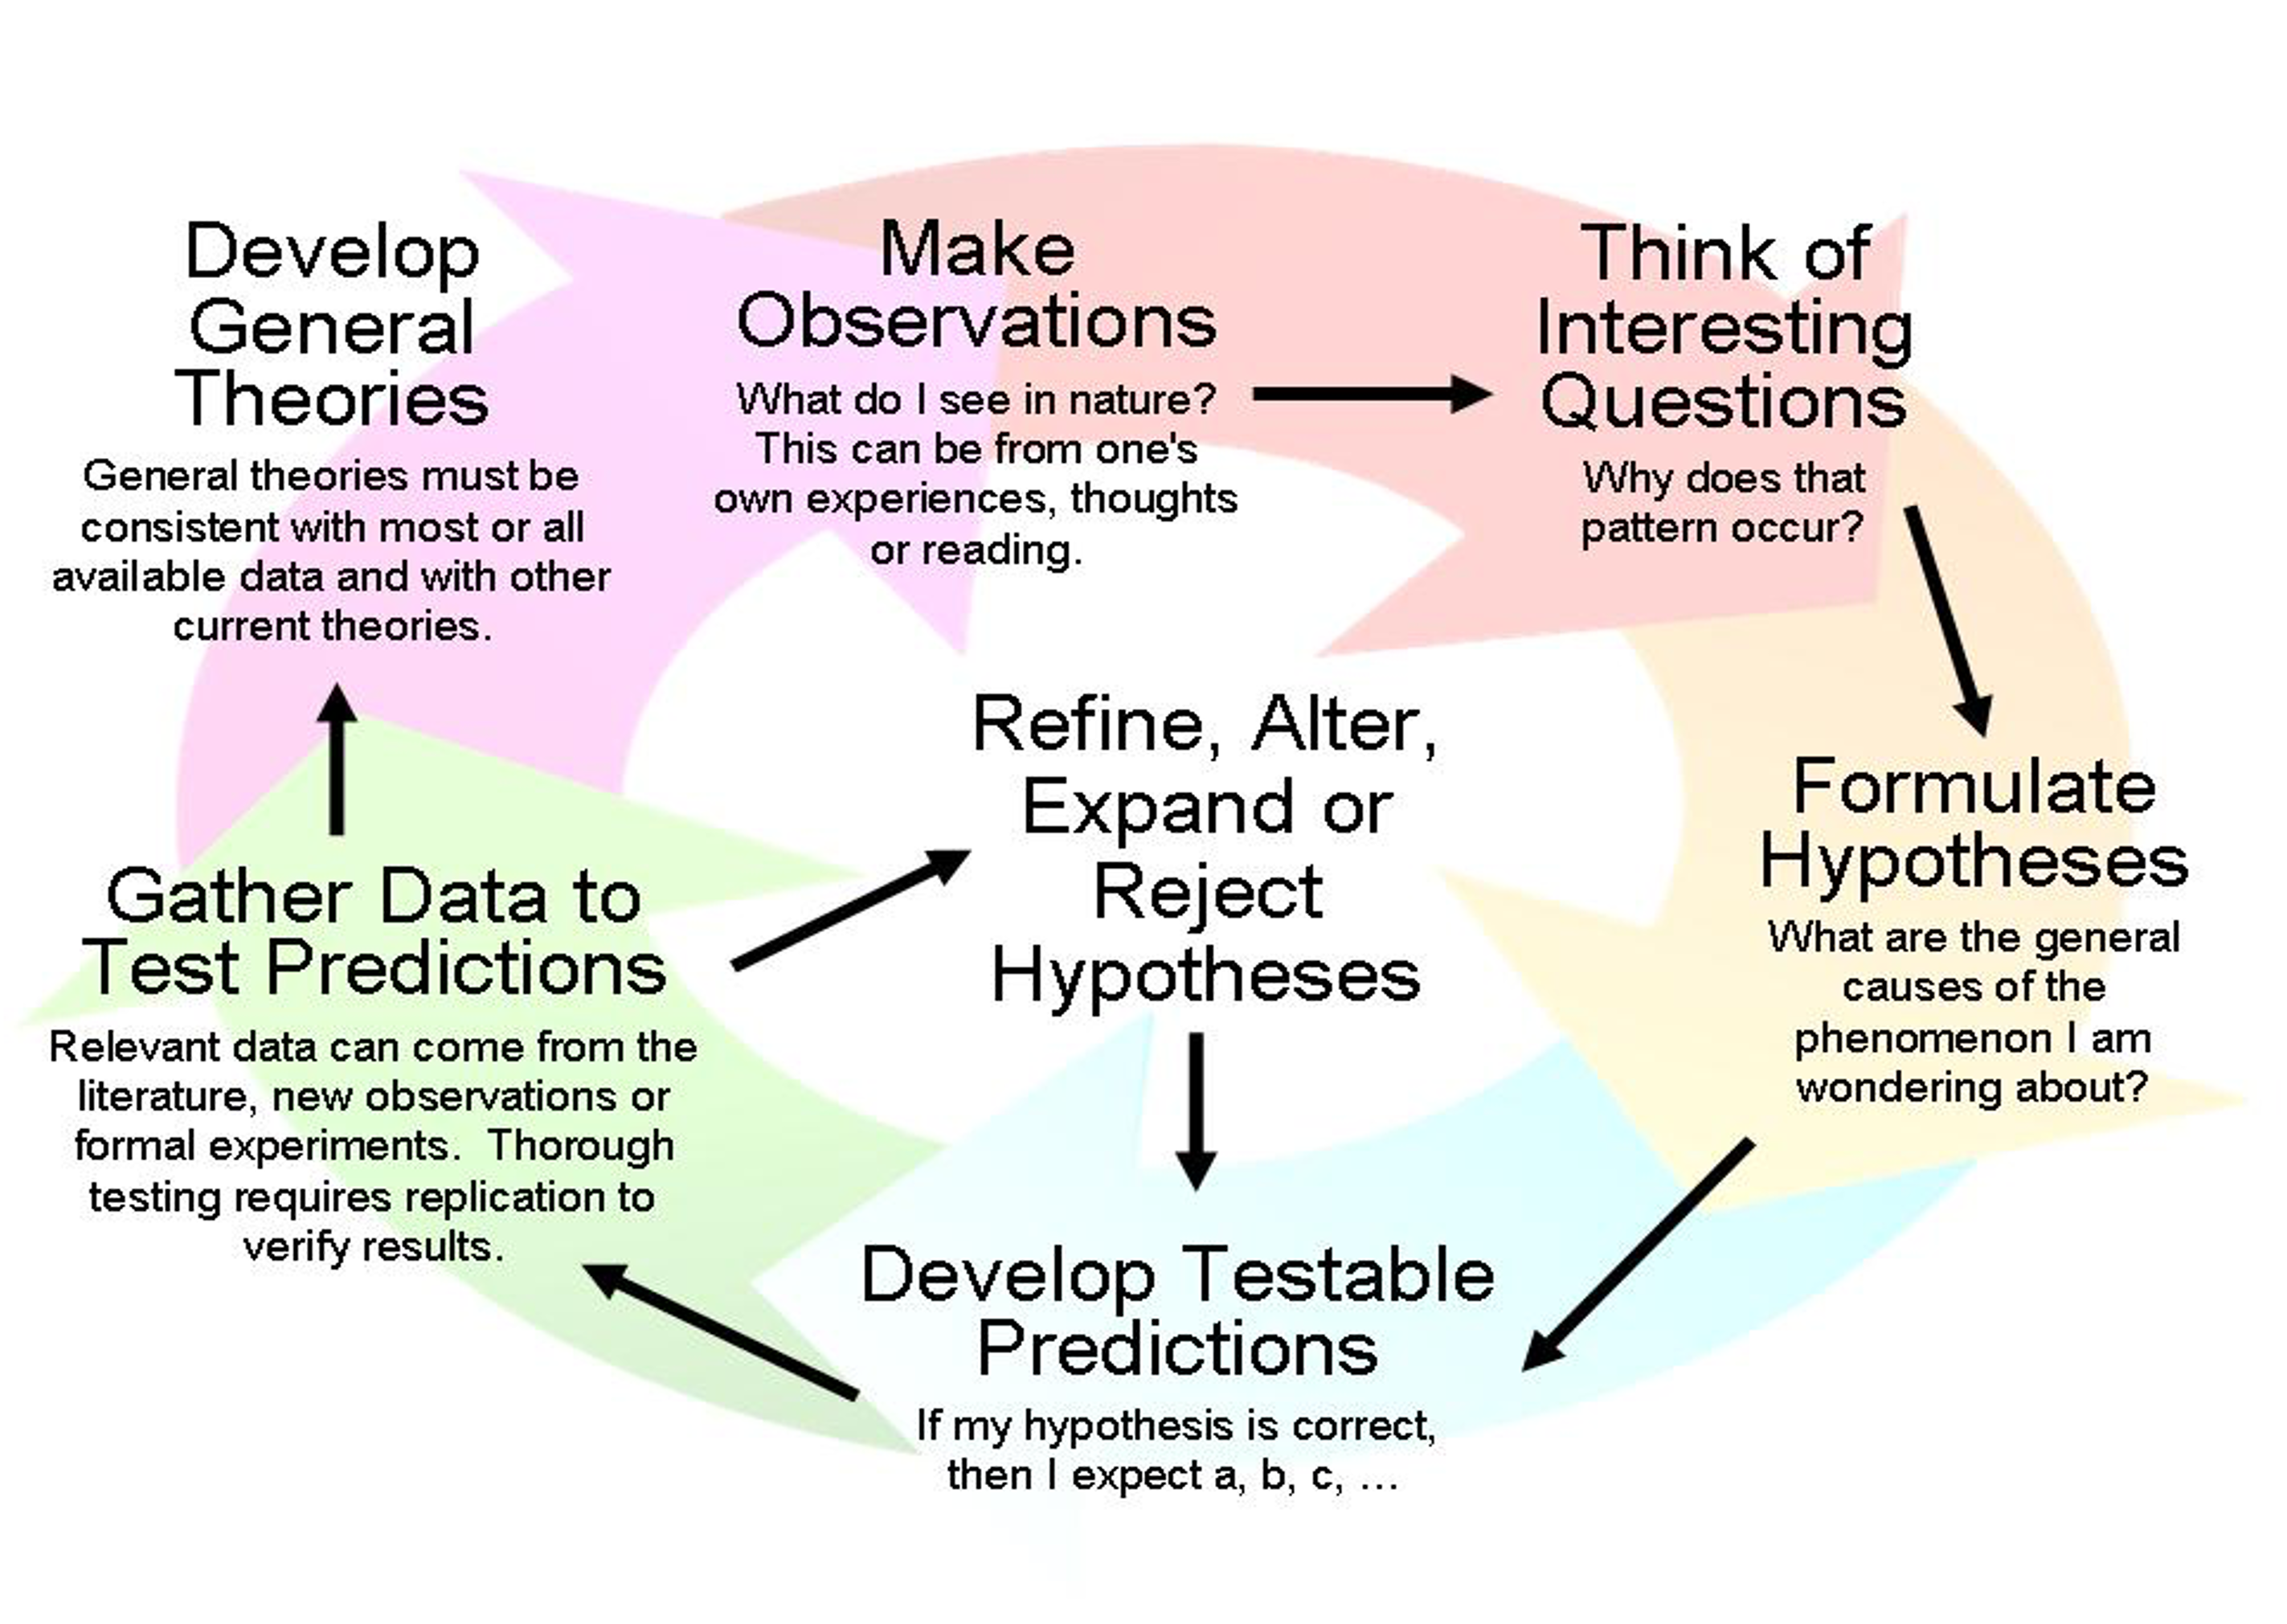
\includegraphics[width=39.53in]{/Users/craig.starbuck/Library/Mobile Documents/com~apple~CloudDocs/Documents/People Analytics Book/GitHub/peopleanalytics_lifecycle_book/graphics/scientific_method} \caption{The Scientific Method}\label{fig:unnamed-chunk-3}
\end{figure}

Over the years, I have adapted the scientific method into a curtailed four-dimensional framework which is intended to elevate the rigor applied to the end-to-end analytical process. The four dimensions are (a) Discover, (b) Design, (c) Develop, and (d) Deliver, and this book will be organized around these. A checklist with general questions and considerations across the analytics lifecycle can be found in the Appendix.

\begin{figure}
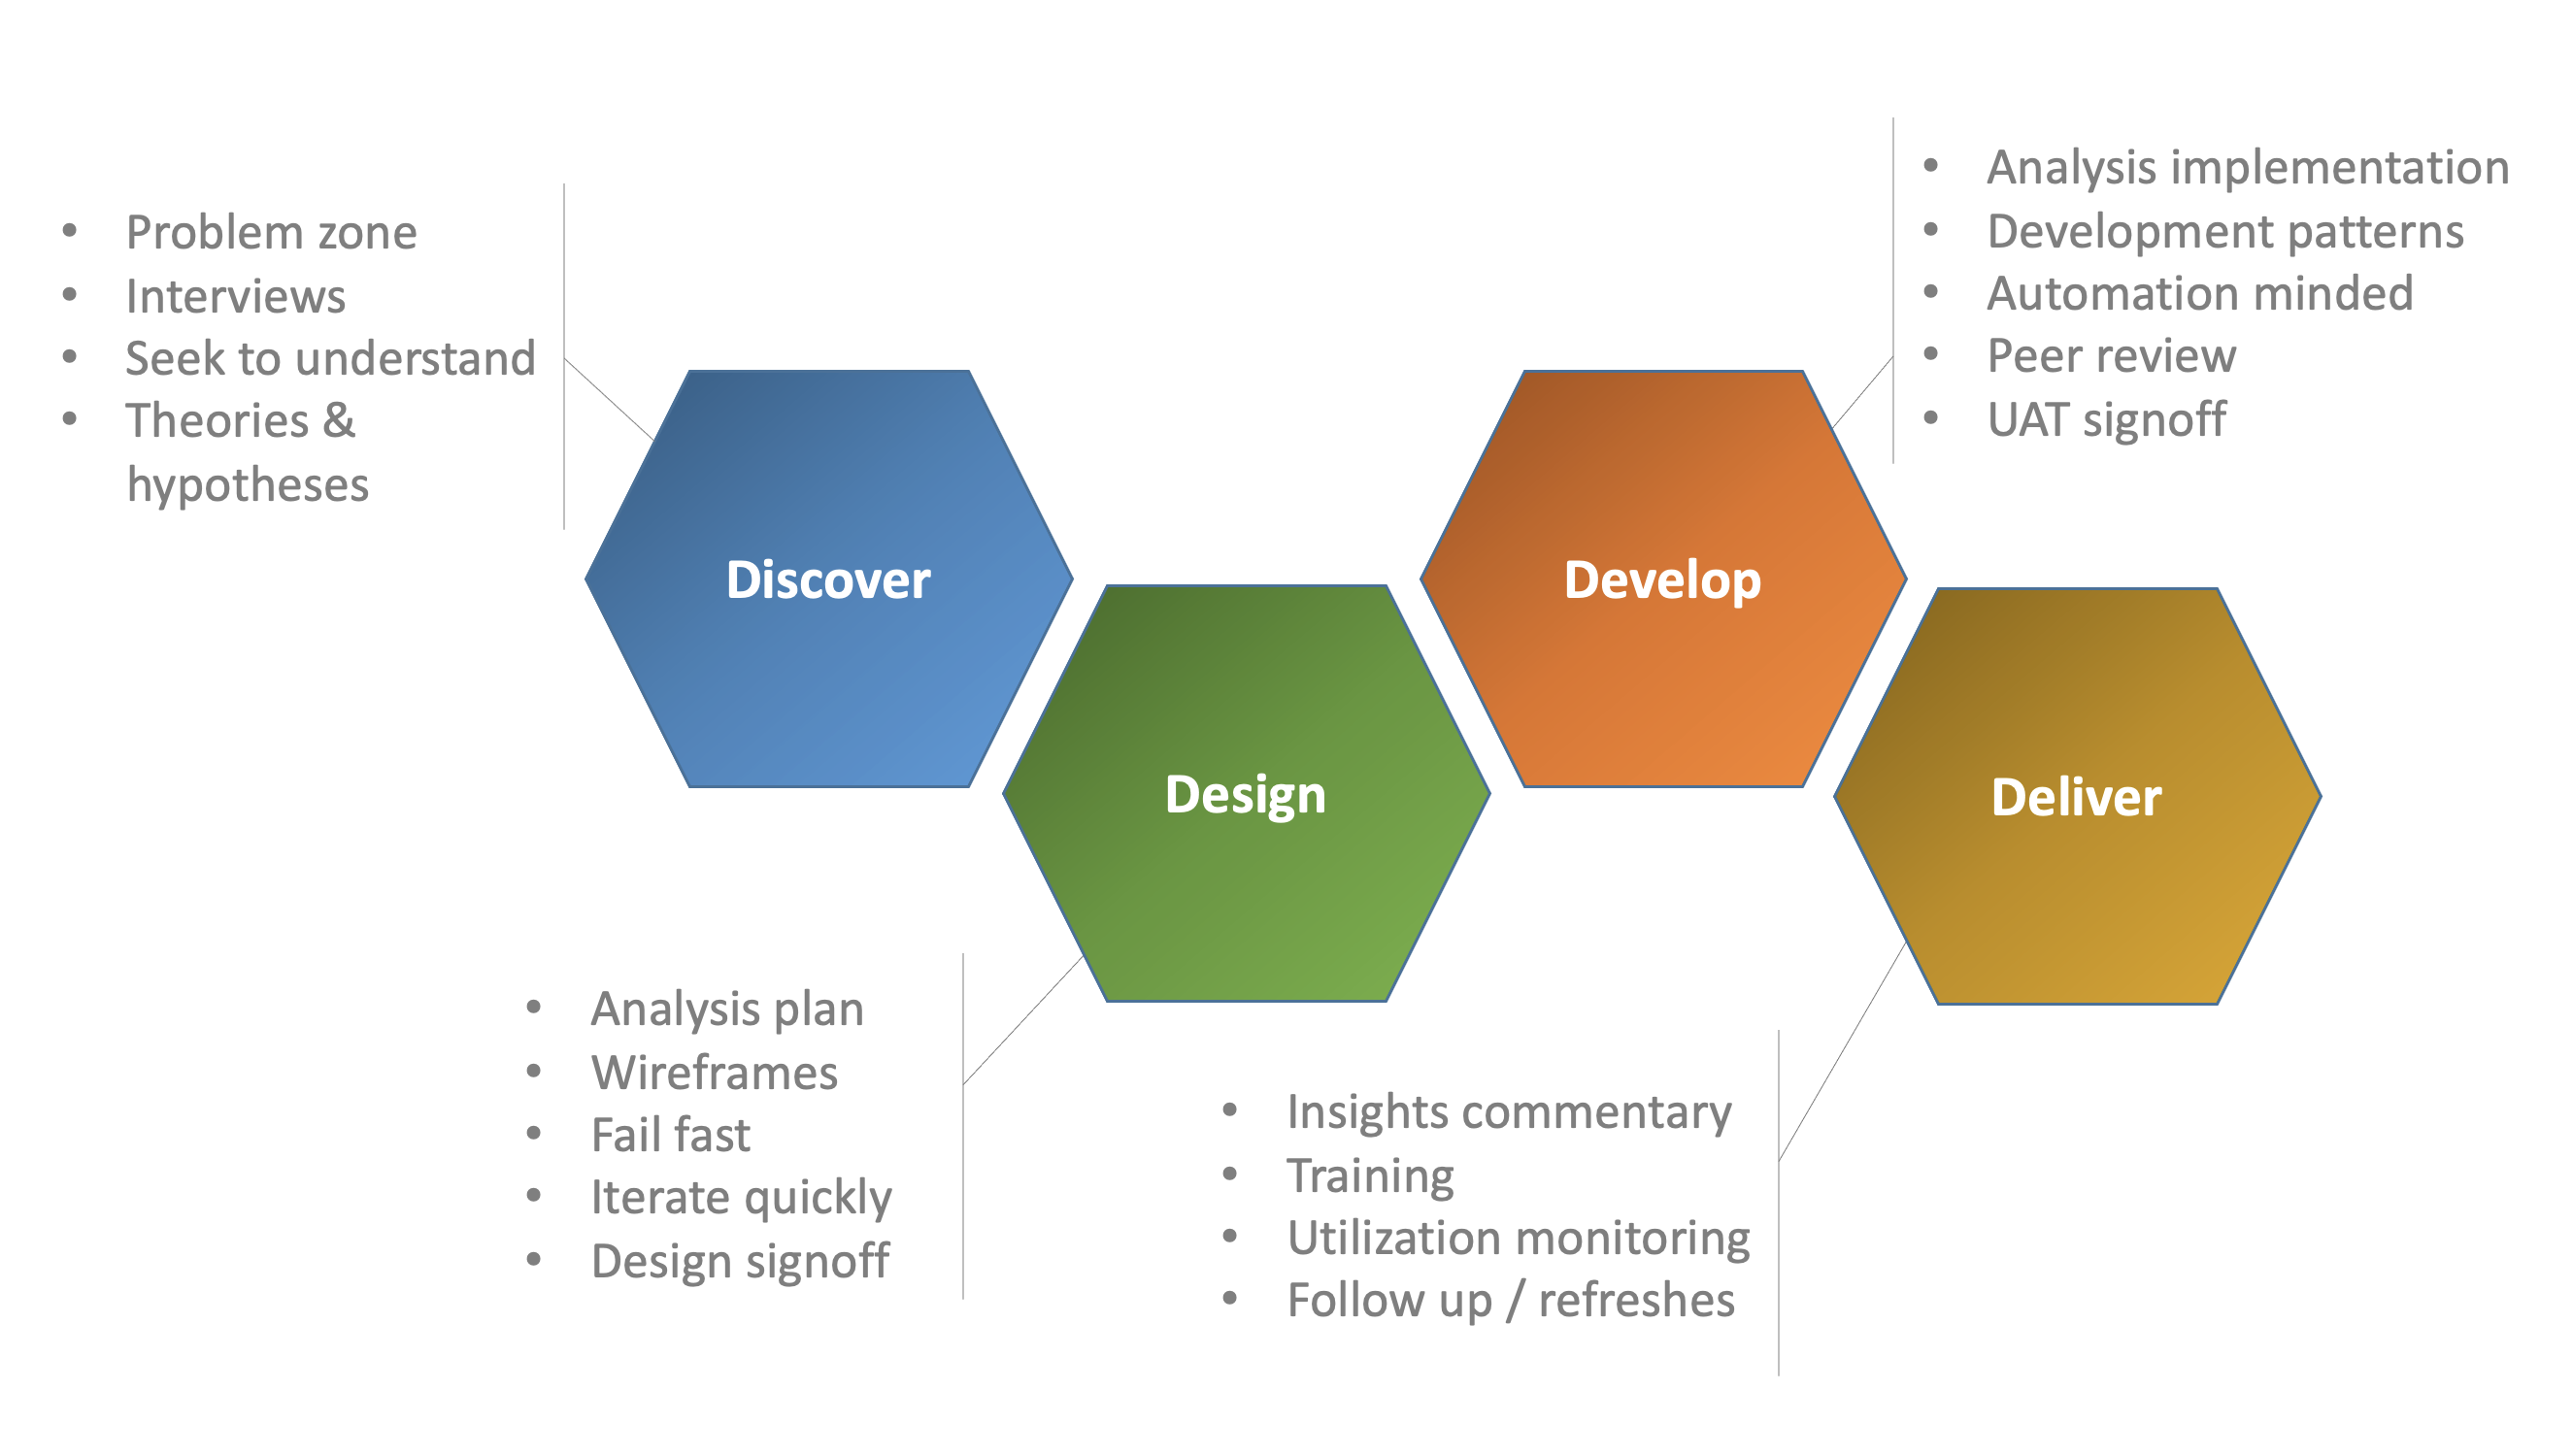
\includegraphics[width=36.81in]{/Users/craig.starbuck/Library/Mobile Documents/com~apple~CloudDocs/Documents/People Analytics Book/GitHub/peopleanalytics_lifecycle_book/graphics/4d_framework_overview} \caption{4D Framework}\label{fig:unnamed-chunk-4}
\end{figure}

1. Discover

You are likely familiar with the old adage: ``An ounce of prevention is worth a pound of cure.'' Such is the case with respect to planning in an analytics context. During the Discover phase, it is important to remain in the problem zone; seek to understand your clients' needs through active listening and questions. This is not the time for solutioning or committing to any specific deliverables. If the client's needs are ambiguous, proceeding will likely be an exercise in futility. Outlined below is a set of general questions that should be considered during this initial phase to prevent allocating scarce time and resourcing to a project that ultimately misses the mark.

2. Design

Perhaps the most important initial question to answer in the design phase is: ``Does anything already exist that addresses part, or all, of the client's objectives?'' If the existing solution will suffice, it's possible that there is simply a communication/education gap, and you can allocate time and resources elsewhere.

The end-user experience is of paramount importance during the Design phase, as solutions should have a consistent look and feel regardless of who developed the product. To achieve this, it is important to resist siloed thinking and consider the broader set of analytics solutions the team has delivered -- or is in the process of delivering.

3. Develop

4. Deliver

The Deliver phase can take many forms depending on the solution being released. If the solution is designed for a large user base, a series of recorded trainings may be in order so that there is a helpful reference for those unable to attend the live sessions or new joiners in the future. It is important to monitor success measures, which could be insights aligned to research hypotheses, dashboard utilization metrics, or any number of others defined within the Discover phase.

\hypertarget{research-methods}{%
\chapter{Research Methods}\label{research-methods}}

\hypertarget{measurement-sampling}{%
\chapter{Measurement \& Sampling}\label{measurement-sampling}}

\hypertarget{populations-samples}{%
\section{Populations \& Samples}\label{populations-samples}}

The goal of research is to understand a population based on data from a subset of population members. In practice, it is often not feasible to collect data from every member of a population, so we instead calculate \textbf{sample statistics} to estimate \textbf{population parameters}.

Another important concept is the \textbf{sampling frame}. While the population represents the entire group of interest, the sampling frame represents the subset of the population to which the researcher has access. In an ideal setting, the population and sampling frame are the same, but they are often different in practice. For example, a professor may be interested in understanding student sentiment about a new school policy but only has access to collect data from students in the courses she teaches. In this case, the entire student body is the population but the students she has access to (those in the courses she teaches) represent the sampling frame. The sample is the subset of the sampling frame that ultimately participates in the research (e.g,. those who complete a survey or participate in a focus group).

\hypertarget{statistical-fundamentals}{%
\chapter{Statistical Fundamentals}\label{statistical-fundamentals}}

This chapter surveys essential univariate, bivariate, and inferential analysis concepts that underpin the more complex multivariate approaches in subsequent chapters of this book.

\hypertarget{univariate-analysis}{%
\section{Univariate Analysis}\label{univariate-analysis}}

\textbf{Descriptive statistics} are rudimentary analysis techniques that help describe and summarize data in a meaningful way. Descriptive statistics do not allow us to draw any conclusions beyond the available data but are helpful in interpreting the data at hand.

There are two categories of descriptive statistics: (a) \textbf{measures of central tendency} describe the central position in a set of data; and (b) \textbf{measures of spread} describe how dispersed the data are.

\hypertarget{measures-of-central-tendency}{%
\subsection{Measures of Central Tendency}\label{measures-of-central-tendency}}

\textbf{Mean}

Perhaps the most intuitive measure of central tendency is the \textbf{mean}, which is often referred to as the average. The mean of a sample is denoted by \(\bar{x}\) and is defined by:

\[ \bar{X} = \frac{\sum_{i=1}^{n} x_{i}}{n} \]

The mean of a set of numeric values can be calculated using the mean() function in R:

\begin{Shaded}
\begin{Highlighting}[]
\CommentTok{# Fill vector x with integers}
\NormalTok{x <-}\StringTok{ }\KeywordTok{c}\NormalTok{(}\DecValTok{1}\NormalTok{,}\DecValTok{1}\NormalTok{,}\DecValTok{1}\NormalTok{,}\DecValTok{2}\NormalTok{,}\DecValTok{2}\NormalTok{,}\DecValTok{2}\NormalTok{,}\DecValTok{3}\NormalTok{,}\DecValTok{3}\NormalTok{,}\DecValTok{4}\NormalTok{,}\DecValTok{50}\NormalTok{)}

\CommentTok{# Calculate average of vector x}
\KeywordTok{mean}\NormalTok{(x)}
\end{Highlighting}
\end{Shaded}

\begin{verbatim}
## [1] 6.9
\end{verbatim}

\textbf{Median}

The \textbf{median} represents the midpoint in a sorted vector of numbers. For vectors with an even number of values, the median is the average of the middle two numbers; it is simply the middle number for vectors with an odd number of values. When the distribution of data is skewed, or there is an extreme value like we observe in vector x, the median is a better measure of central tendency.

The median() function in R can be used to handle the sorting and midpoint selection:

\begin{Shaded}
\begin{Highlighting}[]
\CommentTok{# Calculate median of vector x}
\KeywordTok{median}\NormalTok{(x)}
\end{Highlighting}
\end{Shaded}

\begin{verbatim}
## [1] 2
\end{verbatim}

In this example, the median is only 2 while the mean is 6.9 (which is not really representative of any of the values in vector \(x\)). Large deltas between mean and median values are evidence of outliers.

\textbf{Mode}

The \textbf{mode} is the most frequent number in a set of values.

While mean() and median() are standard functions in R, mode() returns the internal storage mode of the object rather than the statistical mode of the data. We can easily create a function to return the statistical mode(s):

\begin{Shaded}
\begin{Highlighting}[]
\CommentTok{# Create function to calculate statistical mode(s)}
\NormalTok{stat.mode <-}\StringTok{ }\ControlFlowTok{function}\NormalTok{(x) \{}
\NormalTok{  ux <-}\StringTok{ }\KeywordTok{unique}\NormalTok{(x)}
\NormalTok{  tab <-}\StringTok{ }\KeywordTok{tabulate}\NormalTok{(}\KeywordTok{match}\NormalTok{(x, ux))}
\NormalTok{  ux[tab }\OperatorTok{==}\StringTok{ }\KeywordTok{max}\NormalTok{(tab)]}
\NormalTok{\}}

\CommentTok{# Return mode(s) of vector x}
\KeywordTok{stat.mode}\NormalTok{(x)}
\end{Highlighting}
\end{Shaded}

\begin{verbatim}
## [1] 1 2
\end{verbatim}

In this case, we have a bimodal distribution since both 1 and 2 occur most frequently.

\textbf{Range}

The \textbf{range} is the difference between the maximum and minimum values in a set of numbers.

The range() function in R returns the minimum and maximum numbers:

\begin{Shaded}
\begin{Highlighting}[]
\CommentTok{# Return lowest and highest values of vector x}
\KeywordTok{range}\NormalTok{(x)}
\end{Highlighting}
\end{Shaded}

\begin{verbatim}
## [1]  1 50
\end{verbatim}

We can leverage the max() and min() functions to calculate the difference between these values:

\begin{Shaded}
\begin{Highlighting}[]
\CommentTok{# Calculate range of vector x}
\KeywordTok{max}\NormalTok{(x, }\DataTypeTok{na.rm =} \OtherTok{TRUE}\NormalTok{) }\OperatorTok{-}\StringTok{ }\KeywordTok{min}\NormalTok{(x, }\DataTypeTok{na.rm =} \OtherTok{TRUE}\NormalTok{)}
\end{Highlighting}
\end{Shaded}

\begin{verbatim}
## [1] 49
\end{verbatim}

In people analytics, there are many conventional descriptive metrics -- largely counts, percentages, and ratios cut by time series (day, month, quarter, year) and categorical dimensions (department, job, location, tenure band). Here is a sample of common measures:

\begin{itemize}
\tightlist
\item
  Time to Fill: average days between job requisition posting and offer acceptance
\item
  Offer Acceptance Rate: percent of offers extended to candidates that are accepted
\item
  Pass-Through Rate: percent of candidates in a particular stage of the recruiting process who passed through to the next stage
\item
  Progress to Goal: percent of approved positions that have been filled
\item
  cNPS/eNPS: candidate and employee NPS (-100 to 100)
\item
  Headcount: counts and percent of workforce across worker types (employee, intern, contingent)
\item
  Diversity: counts and percent of workforce across gender, ethnicity, and generational cohorts
\item
  Positions: count and percent of open, committed, and filled seats
\item
  Hires: counts and rates
\item
  Career Moves: counts and rates
\item
  Turnover: counts and rates (usually terms / average headcount over the period)
\item
  Workforce Growth: net changes over time, accounting for hires, internal transfers, and exits
\item
  Span of Control: ratio of people leaders to individual contributors
\item
  Layers/Tiers: average and median number of layers removed from CEO
\item
  Engagement: average score or top-box favorability score
\end{itemize}

\hypertarget{measures-of-spread}{%
\subsection{Measures of Spread}\label{measures-of-spread}}

\textbf{Variance}

\textbf{Variance} is a measure of variability in the data. Variance is calculated using the average of squared differences -- or deviations -- from the mean.

Variance of a population is defined by:

\[ \sigma^{2} = \frac{\sum (X_{i}-\mu)^{2}}{N} \]

Variance of a sample is defined by:

\[ s^{2} = \frac{\sum (x_{i}-\bar{x})^{2}}{n-1} \]

It is important to note that since differences are squared, the variance is always non-negative. In addition, we cannot compare these squared differences to the arithmetic mean since the units are different. For example, if we calculate the variance of annual compensation measured in USD, variance should be expressed as USD squared while the mean exists in the original USD unit of measurement.

In R, the sample variance can be calculated using the var() function:

\begin{Shaded}
\begin{Highlighting}[]
\CommentTok{# Load library for data wrangling}
\KeywordTok{library}\NormalTok{(dplyr)}

\CommentTok{# Read employee demographics data}
\NormalTok{demographics <-}\StringTok{ }\KeywordTok{read.csv}\NormalTok{(}\StringTok{"https://raw.githubusercontent.com/crstarbuck/peopleanalytics_lifecycle_book/master/data/files/employee_demographics.csv"}\NormalTok{)}

\CommentTok{# Calculate sample variance for annual compensation}
\KeywordTok{var}\NormalTok{(demographics}\OperatorTok{$}\NormalTok{annual_comp)}
\end{Highlighting}
\end{Shaded}

\begin{verbatim}
## [1] 1876688425
\end{verbatim}

Sample statistics are the default in R. Since the population variance differs from the sample variance by a factor of \texttt{var(x)\ *\ (n\ -\ 1)\ /\ n}, it is simple to convert output from var() to the population variance:

\begin{Shaded}
\begin{Highlighting}[]
\CommentTok{# Store number of observations}
\NormalTok{n =}\StringTok{ }\KeywordTok{nrow}\NormalTok{(demographics)}

\CommentTok{# Calculate population variance for annual compensation}
\KeywordTok{var}\NormalTok{(demographics}\OperatorTok{$}\NormalTok{annual_comp) }\OperatorTok{*}\StringTok{ }\NormalTok{(n }\OperatorTok{-}\StringTok{ }\DecValTok{1}\NormalTok{) }\OperatorTok{/}\StringTok{ }\NormalTok{n}
\end{Highlighting}
\end{Shaded}

\begin{verbatim}
## [1] 1876303464
\end{verbatim}

\textbf{Standard Deviation}

The \textbf{standard deviation} is simply the square root of the variance, as defined by:

\[ s = \sqrt{\frac{\sum (x_{i} - \bar{x})^{2}}{N - 1}} \]

Since a squared value can be converted back to its original units by taking its square root, the standard deviation expresses variability around the mean in the variable's original units.

In R, the sample standard deviation can be calculated using the sd() function:

\begin{Shaded}
\begin{Highlighting}[]
\CommentTok{# Calculate sample standard deviation for annual compensation}
\KeywordTok{sd}\NormalTok{(demographics}\OperatorTok{$}\NormalTok{annual_comp)}
\end{Highlighting}
\end{Shaded}

\begin{verbatim}
## [1] 43320.76
\end{verbatim}

Since the population standard deviation differs from the sample standard deviation by a factor of \texttt{sd(x)\ *\ sqrt((n\ -\ 1)\ /\ n)}, it is simple to convert output from sd() to the population standard deviation:

\begin{Shaded}
\begin{Highlighting}[]
\CommentTok{# Calculate population standard deviation for annual compensation}
\KeywordTok{sd}\NormalTok{(demographics}\OperatorTok{$}\NormalTok{annual_comp) }\OperatorTok{*}\StringTok{ }\KeywordTok{sqrt}\NormalTok{((n }\OperatorTok{-}\StringTok{ }\DecValTok{1}\NormalTok{) }\OperatorTok{/}\StringTok{ }\NormalTok{n)}
\end{Highlighting}
\end{Shaded}

\begin{verbatim}
## [1] 43316.32
\end{verbatim}

\textbf{Quartiles}

\textbf{Quartiles} are a staple of exploratory data analysis (EDA). A quartile is a type of quantile that partitions data into four equally sized parts after ordering the data. Note that each partition is equally sized with respect to the number of data points -- not the range of values in each. Quartiles are also related to \textbf{percentiles}. For example, Q1 is the 25th percentile -- the value at or below which 25\% of values lie. Percentiles are likely more familiar than quartiles, as percentiles show up in the height and weight measurements of babies, performance on standardized tests like the SAT and GRE, among other things.

The \textbf{Interquartile Range (IQR)} represents the difference between Q3 and Q1 cut point values (the middle two quartiles). The IQR is sometimes used to detect extreme values in a distribution; values less than \(Q1 - 1.5 * IQR\) or greater than \(Q3 + 1.5 * IQR\) are generally considered outliers.

In R, the quantile() function returns the values that bookend each quartile:

\begin{Shaded}
\begin{Highlighting}[]
\CommentTok{# Return quartiles for annual compensation}
\KeywordTok{quantile}\NormalTok{(demographics}\OperatorTok{$}\NormalTok{annual_comp)}
\end{Highlighting}
\end{Shaded}

\begin{verbatim}
##       0%      25%      50%      75%     100% 
##  50016.0  87946.0 125522.0 163262.5 199968.0
\end{verbatim}

Based on this output, we know that 25\% of people in our data earn annual compensation of 87,946 USD or less, 125,522 USD is the median annual compensation, and 75\% of people earn annual compensation of 163,263 USD or less.

We can also return a specific percentile value using the \texttt{probs} argument in the quantile() function. For example, if we want to know the 80th percentile annual compensation value, we can execute the following:

\begin{Shaded}
\begin{Highlighting}[]
\CommentTok{# Return 80th percentile annual compensation value}
\KeywordTok{quantile}\NormalTok{(demographics}\OperatorTok{$}\NormalTok{annual_comp, }\DataTypeTok{probs =} \FloatTok{.8}\NormalTok{)}
\end{Highlighting}
\end{Shaded}

\begin{verbatim}
##      80% 
## 170196.4
\end{verbatim}

In addition, the summary() function returns several common descriptive statistics for an object:

\begin{Shaded}
\begin{Highlighting}[]
\CommentTok{# Return common descriptives}
\KeywordTok{summary}\NormalTok{(demographics}\OperatorTok{$}\NormalTok{annual_comp)}
\end{Highlighting}
\end{Shaded}

\begin{verbatim}
##    Min. 1st Qu.  Median    Mean 3rd Qu.    Max. 
##   50016   87946  125522  125369  163262  199968
\end{verbatim}

\hypertarget{bivariate-analysis}{%
\subsection{Bivariate Analysis}\label{bivariate-analysis}}

\textbf{Covariance}

While variance provides an understanding of how values for a single variable vary, \textbf{covariance} is an unstandardized measure of how two variables vary together. Values can range from \(-\infty\) to \(+\infty\), and these values can be used to understand the direction of the linear relationship between variables. Positive covariance values indicate that the variables vary in the same direction (e.g., tend to increase or decrease together), while negative covariance values indicate that the variables vary in opposite directions (e.g., when one increases, the other decreases, or vice versa).

Covariance of a sample is defined by:

\[ cov_{x,y} = \frac{\sum(x_{i}-\bar{x})(y_{i}-\bar{y})}{N-1} \]

It's important to note that while covariance aids our understanding of the direction of the relationship between two variables, we cannot use it to understand the strength of the association since it is unstandardized. Due to differences in variables' units of measurement, the strength of the relationship between two variables with large covariance could be weak, while the strength of the relationship between another pair of variables with small covariance could be strong.

In R, we can compute the covariance between a pair of numeric variables by passing the two vectors into the cov() function:

\begin{Shaded}
\begin{Highlighting}[]
\CommentTok{# Calculate sample covariance between annual compensation and age using complete observations (missing values will cause issues if not addressed)}
\KeywordTok{cov}\NormalTok{(demographics}\OperatorTok{$}\NormalTok{annual_comp, demographics}\OperatorTok{$}\NormalTok{age, }\DataTypeTok{use =} \StringTok{"complete.obs"}\NormalTok{)}
\end{Highlighting}
\end{Shaded}

\begin{verbatim}
## [1] 453179.1
\end{verbatim}

In this example, using the default Pearson method, the covariance between annual compensation and age is 453179.1. The positive value indicates that annual compensation is generally higher for older employees and lower for younger employees.

Just as we multiplied the sample variance by \((n - 1) / n\) to obtain the population variance, we can apply the same approach to convert the sample covariance returned by cov() to the population covariance:

\begin{Shaded}
\begin{Highlighting}[]
\CommentTok{# Calculate population covariance between annual compensation and age}
\KeywordTok{cov}\NormalTok{(demographics}\OperatorTok{$}\NormalTok{annual_comp, demographics}\OperatorTok{$}\NormalTok{age, }\DataTypeTok{use =} \StringTok{"complete.obs"}\NormalTok{) }\OperatorTok{*}\StringTok{ }\NormalTok{(n }\OperatorTok{-}\StringTok{ }\DecValTok{1}\NormalTok{) }\OperatorTok{/}\StringTok{ }\NormalTok{n}
\end{Highlighting}
\end{Shaded}

\begin{verbatim}
## [1] 453086.1
\end{verbatim}

The examples thus far have only examined associations between two variables at a time. However, rather than looking at isolated pairwise relationships, we can produce a covariance matrix to surface associations among many variables by passing a dataframe or matrix object into the cov() function:

\begin{Shaded}
\begin{Highlighting}[]
\CommentTok{# Generate a correlation matrix among continuous variables}
\KeywordTok{cov}\NormalTok{(demographics[, }\KeywordTok{c}\NormalTok{(}\StringTok{"annual_comp"}\NormalTok{, }\StringTok{"age"}\NormalTok{, }\StringTok{"org_tenure"}\NormalTok{, }\StringTok{"job_tenure"}\NormalTok{)], }\DataTypeTok{use =} \StringTok{"complete.obs"}\NormalTok{)}
\end{Highlighting}
\end{Shaded}

\begin{verbatim}
##              annual_comp          age   org_tenure  job_tenure
## annual_comp 1.876688e+09 453179.07281 138551.67644 61576.73603
## age         4.531791e+05    168.38661     41.56006    17.96902
## org_tenure  1.385517e+05     41.56006     26.03270    11.04572
## job_tenure  6.157674e+04     17.96902     11.04572    13.29996
\end{verbatim}

Using the default Pearson method, the cov() function will return sample variances for each variable down the diagonal, since covariance is not applicable in the context of a variable with itself. We can confirm by producing the variance for age:

\begin{Shaded}
\begin{Highlighting}[]
\CommentTok{# Return sample variance for age}
\KeywordTok{var}\NormalTok{(demographics}\OperatorTok{$}\NormalTok{age)}
\end{Highlighting}
\end{Shaded}

\begin{verbatim}
## [1] 168.3866
\end{verbatim}

As expected, the variance for age (\(s^{2}\) = 168.39) matches the value found in the age x age cell of the covariance matrix.

\textbf{Correlation}

\textbf{Correlation} is a scaled form of covariance. While covariance provides an unstandardized measure of the direction of a relationship between variables, correlation provides a standardized measure that can be used to quantify both the direction and strength of bivariate relationships. Correlation coefficients range from -1 to 1, where -1 indicates a perfectly negative association, 1 indicates a perfectly positive association, and 0 indicates the absence of an association. \textbf{Pearson's product-moment correlation coefficient} \(r\) is defined by:

\[ r_{x,y} = \frac{\sum(x_{i}-\bar{x})(y_{i}-\bar{y})}{\sqrt{\sum_(x_{i}-\bar{x})^2\sum_(y_{i}-\bar{y})^2}} \]

In R, Pearson's \(r\) can be calculated using the cor() function:

\begin{Shaded}
\begin{Highlighting}[]
\CommentTok{# Calculate the correlation between annual compensation and age}
\KeywordTok{cor}\NormalTok{(demographics}\OperatorTok{$}\NormalTok{annual_comp, demographics}\OperatorTok{$}\NormalTok{age, }\DataTypeTok{use =} \StringTok{"complete.obs"}\NormalTok{)}
\end{Highlighting}
\end{Shaded}

\begin{verbatim}
## [1] 0.8061577
\end{verbatim}

While we already know that the relationship between annual compensation and age is positive based on the positive covariance coefficient, Pearson's \(r\) of .81 indicates that the strength of the positive association is strong (\(r\) = 1 is perfectly positive). Though there are no absolute rules for categorizing the strength of relationships, as thresholds often vary by domain, the following is a general rule of thumb for interpreting the strength of bivariate associations:

\begin{itemize}
\tightlist
\item
  Weak = Absolute value of correlation coefficients between 0 and .3
\item
  Moderate = Absolute value of correlation coefficients between .4 and .6
\item
  Strong = Absolute value of correlation coefficients between .7 and 1
\end{itemize}

There are several correlation coefficients, and the measurement scale of \(x\) and \(y\) determine the appropriate type:

\begin{figure}

{\centering 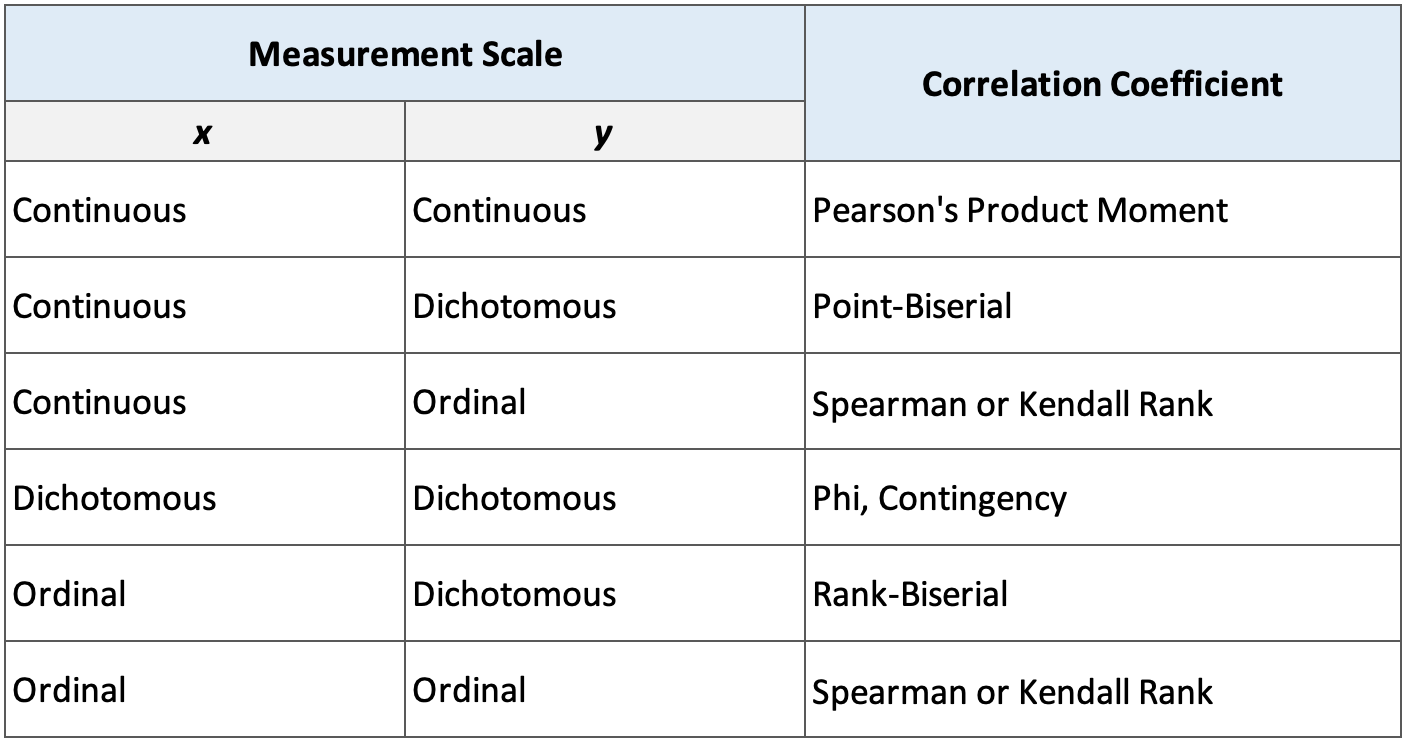
\includegraphics[width=19.56in]{/Users/craig.starbuck/Library/Mobile Documents/com~apple~CloudDocs/Documents/People Analytics Book/GitHub/peopleanalytics_lifecycle_book/graphics/correlation_table} 

}

\caption{Proper Applications of Correlation Coefficients}\label{fig:unnamed-chunk-22}
\end{figure}

Pearson's \(r\) can be used when both variables are measured on continuous scales or when one is continuous and the other is dichotomous (point-biserial correlation).

When one or both variables are ordinal, we can leverage \textbf{Spearman's} \(\rho\) or \textbf{Kendall's} \(\tau\), which are both standardized nonparametric measures of the association between one or two rank-ordered variables. Let's look at Spearman's \(\rho\), which is defined as:

\[ \rho = 1 - {\frac {6 \sum d_i^2}{n(n^2 - 1)}} \]

We can override the default Pearson method in the cor() function to implement a specific form of rank correlation using the \texttt{method} argument:

\begin{Shaded}
\begin{Highlighting}[]
\CommentTok{# Calculate the correlation between job level and education level using Spearman's method}
\KeywordTok{cor}\NormalTok{(demographics}\OperatorTok{$}\NormalTok{job_level, demographics}\OperatorTok{$}\NormalTok{education, }\DataTypeTok{method =} \StringTok{"spearman"}\NormalTok{, }\DataTypeTok{use =} \StringTok{"complete.obs"}\NormalTok{)}
\end{Highlighting}
\end{Shaded}

\begin{verbatim}
## [1] 0.6749776
\end{verbatim}

The \(\rho\) coefficient of .67 indicates that the positive association we observed between job level and education level is moderate-to-strong. We could also pass \texttt{method\ =\ "kendall"} to this cor() function to implement Kendall's \(\tau\).

The \textbf{Phi Coefficient} (\(\phi\)), sometimes referred to as the mean square contingency coefficient or Matthews correlation in ML, can be used to understand the association between two dichotomous variables. For a 2x2 table for two random variables \(x\) and \(y\):

\begin{figure}

{\centering 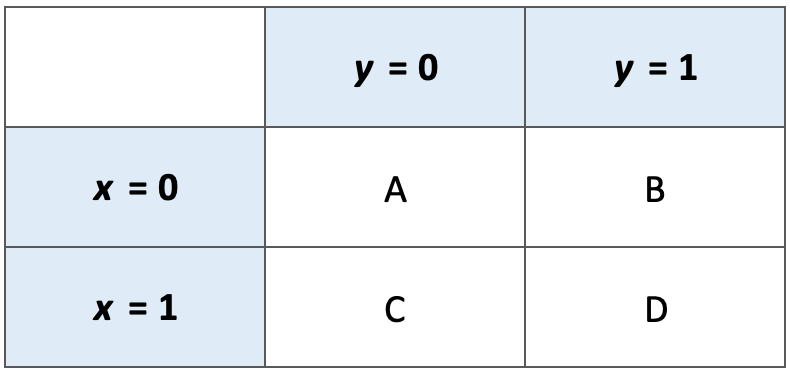
\includegraphics[width=10.97in]{/Users/craig.starbuck/Library/Mobile Documents/com~apple~CloudDocs/Documents/People Analytics Book/GitHub/peopleanalytics_lifecycle_book/graphics/phi_coefficient_formula} 

}

\caption{2x2 Table for Random Variables x and y}\label{fig:unnamed-chunk-24}
\end{figure}

The \(\phi\) coefficient is defined as:

\[ \phi = {\frac {(AD-BC)}{\sqrt{(A+B)(C+D)(A+C)(B+D)}}} \]

To illustrate, let's examine whether there is a relationship between gender and performance after transforming performance from its ordinal form to a dichotomous variable (high vs.~low performance). We can leverage the \texttt{psych} library to calculate \(\phi\) in R:

\begin{Shaded}
\begin{Highlighting}[]
\CommentTok{# Load library for Phi Coefficient}
\KeywordTok{library}\NormalTok{(psych)}

\CommentTok{# Set females to 1 and everything else to 0}
\NormalTok{demographics}\OperatorTok{$}\NormalTok{gender_code <-}\StringTok{ }\KeywordTok{ifelse}\NormalTok{(demographics}\OperatorTok{$}\NormalTok{gender }\OperatorTok{==}\StringTok{ 'Female'}\NormalTok{, }\DecValTok{1}\NormalTok{, }\DecValTok{0}\NormalTok{)}

\CommentTok{# Set high performers (3 and above) to 1 and everything else to 0}
\NormalTok{demographics}\OperatorTok{$}\NormalTok{performance_code <-}\StringTok{ }\KeywordTok{ifelse}\NormalTok{(demographics}\OperatorTok{$}\NormalTok{performance }\OperatorTok{<}\StringTok{ }\DecValTok{3}\NormalTok{, }\DecValTok{0}\NormalTok{, }\DecValTok{1}\NormalTok{)}

\CommentTok{# Create a 2x2 contingency table}
\NormalTok{contingency_tbl <-}\StringTok{ }\KeywordTok{table}\NormalTok{(demographics}\OperatorTok{$}\NormalTok{gender_code, demographics}\OperatorTok{$}\NormalTok{performance_code)}

\CommentTok{# Calculate the Phi Coefficient between dichotomous variables}
\KeywordTok{phi}\NormalTok{(contingency_tbl)}
\end{Highlighting}
\end{Shaded}

\begin{verbatim}
## [1] 0.01
\end{verbatim}

\(\phi\) is essentially 0, which means performance ratings are distributed equitably across gender categories (good news!).

A correlation matrix can be produced to surface associations among many variables by passing a dataframe or matrix object into the cor() function:

\begin{Shaded}
\begin{Highlighting}[]
\CommentTok{# Generate a correlation matrix among continuous variables}
\KeywordTok{cor}\NormalTok{(demographics[, }\KeywordTok{c}\NormalTok{(}\StringTok{"annual_comp"}\NormalTok{, }\StringTok{"age"}\NormalTok{, }\StringTok{"org_tenure"}\NormalTok{, }\StringTok{"job_tenure"}\NormalTok{)], }\DataTypeTok{use =} \StringTok{"complete.obs"}\NormalTok{)}
\end{Highlighting}
\end{Shaded}

\begin{verbatim}
##             annual_comp       age org_tenure job_tenure
## annual_comp   1.0000000 0.8061577  0.6268392  0.3897584
## age           0.8061577 1.0000000  0.6277154  0.3797042
## org_tenure    0.6268392 0.6277154  1.0000000  0.5936211
## job_tenure    0.3897584 0.3797042  0.5936211  1.0000000
\end{verbatim}

Based on this correlation matrix, there are several moderate and strong pairwise associations in the data. The values down the diagonal are 1 because these represent the correlation between each variable and itself. You may also notice that the information above and below the diagonal is identical and, therefore, redundant.

A great R library for visualizing correlation matrices is corrplot. Several arguments can be specified for various visual representations of the relationships among variables:

\begin{Shaded}
\begin{Highlighting}[]
\CommentTok{# Load library for correlation visuals}
\KeywordTok{library}\NormalTok{(corrplot)}

\CommentTok{# Store correlation matrix to object M}
\NormalTok{M <-}\StringTok{ }\KeywordTok{cor}\NormalTok{(demographics[, }\KeywordTok{c}\NormalTok{(}\StringTok{"annual_comp"}\NormalTok{, }\StringTok{"age"}\NormalTok{, }\StringTok{"org_tenure"}\NormalTok{, }\StringTok{"job_tenure"}\NormalTok{)], }\DataTypeTok{method =} \StringTok{"spearman"}\NormalTok{, }\DataTypeTok{use =} \StringTok{"complete.obs"}\NormalTok{)}

\CommentTok{# Visualize correlation matrix}
\KeywordTok{corrplot.mixed}\NormalTok{(M, }\DataTypeTok{order =} \StringTok{'AOE'}\NormalTok{)}
\end{Highlighting}
\end{Shaded}

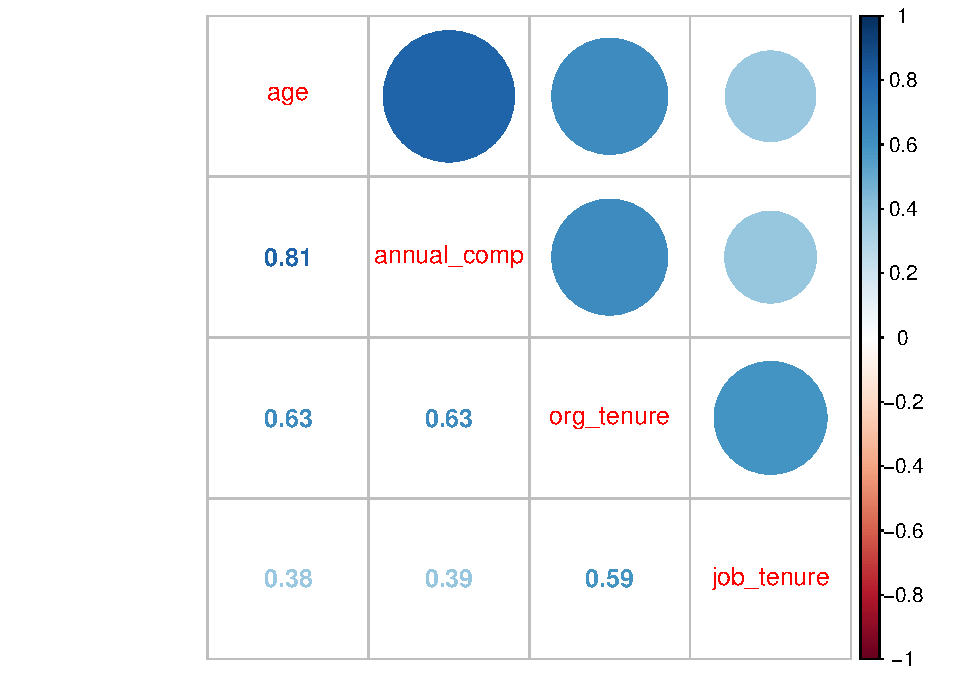
\includegraphics{_main_files/figure-latex/unnamed-chunk-27-1.pdf}

It's important to remember that correlation is not causation. Correlations can be spurious (variables related by chance), and drawing conclusions based on bivariate associations alone -- especially in the absence of sound theoretical underpinnings -- can be dangerous. Here are two examples of nearly perfect correlations between variables for which there is likely no true direct association:

\begin{figure}

{\centering 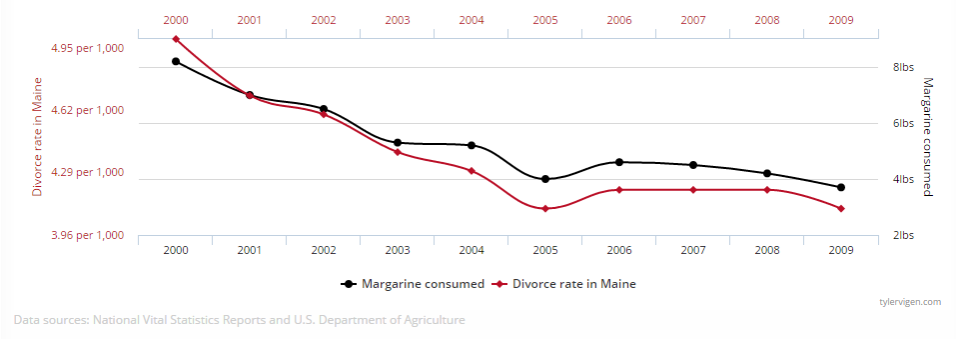
\includegraphics[width=13.28in]{/Users/craig.starbuck/Library/Mobile Documents/com~apple~CloudDocs/Documents/People Analytics Book/GitHub/peopleanalytics_lifecycle_book/graphics/spurious_corr_maine_divorce} 

}

\caption{Correlation between Maine Divorce Rate and Margarine Consumption (r = .99)}\label{fig:unnamed-chunk-28}
\end{figure}

\begin{figure}

{\centering 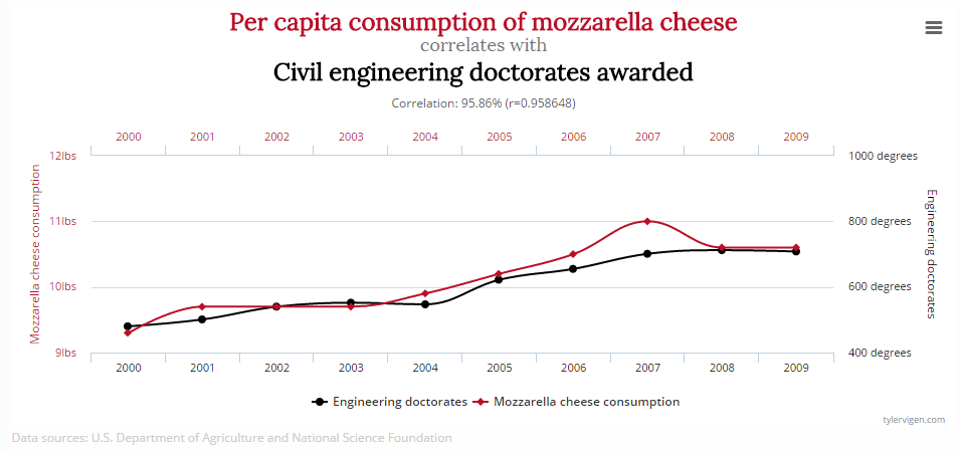
\includegraphics[width=13.29in]{/Users/craig.starbuck/Library/Mobile Documents/com~apple~CloudDocs/Documents/People Analytics Book/GitHub/peopleanalytics_lifecycle_book/graphics/spurious_corr_mozzarella_cheese} 

}

\caption{Correlation between Mozzarella Cheese Consumption and Civil Engineering Doctorate Conferrals (r = .96)}\label{fig:unnamed-chunk-29}
\end{figure}

In addition, covariance and correlation alone are not sufficient for determining whether an observed association in sample data is also present in the population. To understand the likelihood that patterns observed in sample data are also present in the larger population of interest, we need to move beyond descriptive measures.

\hypertarget{inferential-statistics}{%
\section{Inferential Statistics}\label{inferential-statistics}}

The objective of \textbf{inferential statistics} is to make inferences -- with some degree of confidence -- about a population based on available sample data. Several related concepts underpin this goal and will be covered here.

\hypertarget{introduction-to-probability}{%
\subsection{Introduction to Probability}\label{introduction-to-probability}}

\textbf{Randomness} and uncertainty exist all around us. In \textbf{probability theory}, random phenomena refers to events or experiments whose outcomes cannot be predicted with certainty (Pishro-Nik, 2014). If you've taken a course in probability, there is a good chance you have considered the case of a fair coin flip -- one of the most intuitive applications of probability. In the absence of information on how the coin is flipped, we cannot be certain of the outcome. What we can be certain of is that with a large number of coin flips, the proportion of heads will become increasingly close to 50\%, or \(\frac{1}{2}\).

The \textbf{Law of Large Numbers (LLN)} is an important theorem for building an intuitive understanding of how probability relates to the statistical inference concepts we will cover. In the case of a fair coin flip, it is possible to observe many consecutive heads by chance. This is because small samples can lend to anamalies. However, as the number of flips increases, we will undoubtedly observe an increasing number of tails; we expect a roughly equal number of heads and tails with a large enough number of flips.

\textbf{Conditional probability} reflects the probability conditioned on the occurrence of a previous event or outcome. For example, we may find that the proportion of heads is greater or less than \(\frac{1}{2}\) with a large number of fair coin flips when the coin is consistently heads up when flipped. The outcome is, therefore, conditioned on the fixed -- rather than random -- positioning of the coin when flipped.

Formally, \textbf{Bayes' Theorem (alternatively, Bayes' Rule)} states that for any two events A and B where the probability of A is not 0 (\(P(A) \neq 0\)):

\[ P(B \vert A) = \frac{P(A \vert B) P(B)}{P(A)} \]

Bayes' Rule allows us to more accurately predict the outcome by conditioning the probability on known factors rather than assuming all events operate under the same conditions. Bayes' Rule is pervasive in people analytics, as the probability of outcomes can vary widely based on a person's age, tenure, education, job, perceptions, relationships, and many other factors. For example, if we consider a company with 100 terminations over a 12-month period and average headcount of 1,000, the probability of attrition not conditioned on any other factor is 10\%, or \(\frac{1}{10}\). Aside from trending this probability over time to identify if attrition is becoming more or less of a concern, this isn't too helpful at the broader company level. However, if we condition the probability of attrition on an event -- such as a recent manager exit -- and find that the probability of attrition among those whose manager has left in the last six months is 70\%, or \(\frac{7}{10}\), this is far more actionable (and concerning).

\hypertarget{central-limit-theorem}{%
\subsection{Central Limit Theorem}\label{central-limit-theorem}}

The \textbf{Central Limit Theorem (CLT)} is a mainstay of statistics and probability and fundamental to understanding the mechanics of multivariate inferential analysis techniques we will cover later in this book. The CLT was initially coined by a French-born mathematician named Abraham De Moivre in the 1700s. While initially unpopular, it was later reintroduced and attracted new interest from theorists and academics (Daw \& Pearson, 1972).

The CLT states that the average of independent random variables, when increased in number, tend to follow a normal (or Gaussian) distribution. The distribution of sample means approaches a normal distribution regardless of the shape of the population distribution from which the samples are drawn. This is important because the normal distribution has properties that can be used to test the likelihood that an observed value, difference, or relationship in a sample is also present in the population.

\begin{figure}

{\centering 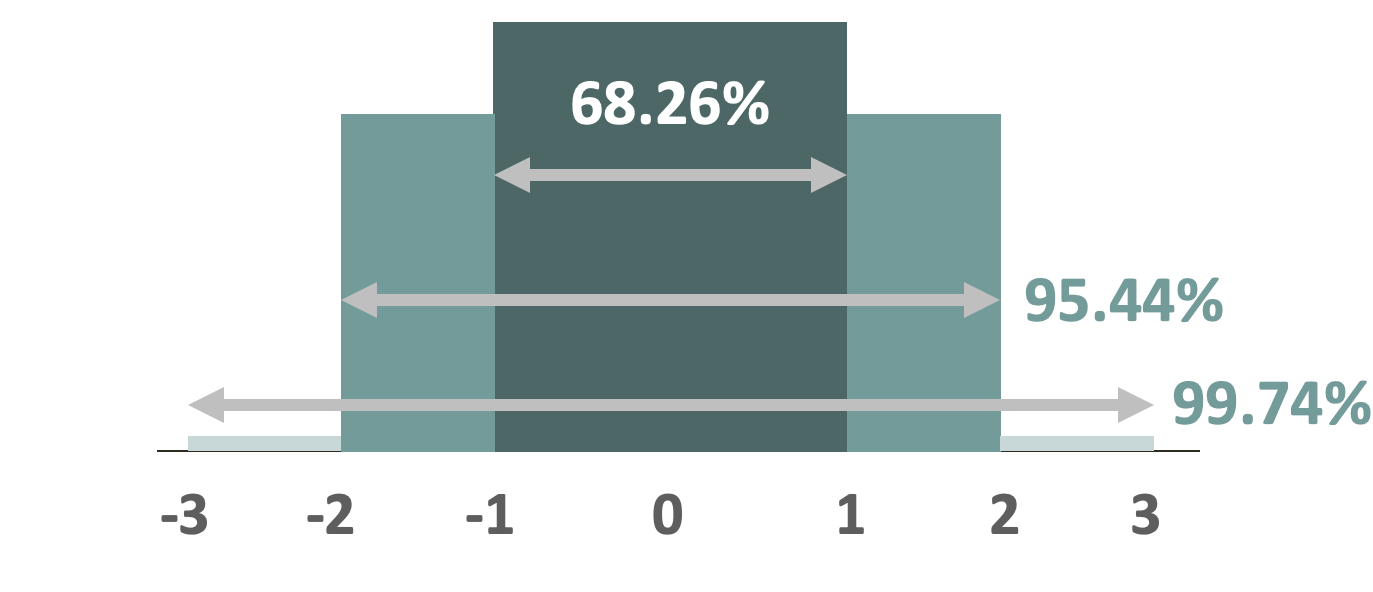
\includegraphics[width=19.07in]{/Users/craig.starbuck/Library/Mobile Documents/com~apple~CloudDocs/Documents/People Analytics Book/GitHub/peopleanalytics_lifecycle_book/graphics/normal_distribution} 

}

\caption{The Empirical Rule}\label{fig:unnamed-chunk-30}
\end{figure}

Let's begin with an intuitive example of CLT. Imagine that we have a reliable way to measure how fun a population is on a 100-point scale, where 100 indicates maximum fun (life of the party) and 1 indicates maximum boringness. Consider that a small statistics conference is in progress at a nearby convention center, and there are 40 statisticians in attendance. In a separate room at the same convention center, there is also a group of 40 random people (non-statisticians) who are gathered to discuss some less interesting topic. Our job is to walk into one of the rooms and determine -- on the basis of the ``fun'' factor alone -- whether we have entered the statistics conference or the other, less interesting gathering of non-statisticians.

Let's assume the mean fun score and standard deviation of these two groups are known; the group of statisticians have, on average, a fun score of 85 with a standard deviation of 2, while the group of non-statisticians are a bit less fun with a mean score of 65 and a standard deviation of 4. With a known population mean and standard deviation, the standard error (the standard deviation of the sample means) provides the ability to calculate the probability that the sample (the room of 40 people) belongs to the population of interest (fellow statisticians).

Herein lies the beauty of the CLT: roughly 68 percent of sample means will lie within one standard error of the population mean, roughly 95 percent within two standard errors of the population mean, and roughly 99 percent within three standard errors of the population mean. Therefore, any room whose members have an average fun score that is not within two standard errors of the population mean (between 81 and 89 for our statisticians) is statistically unlikely to be the group of statisticians for which we are searching. This is because in less than 5 in 100 cases could we randomly draw a `reasonably sized' sample of statisticians with average funness so extremely different from the population average.

Because small samples lend to anomalies, we could -- by chance -- select a single person who happens to fall in the tails (extremely boring or extremely fun); however, as the sample size increases, it becomes more and more likely that the observed average reflects the average of the larger population. It would be virtually impossible (in less than 1 in 100 cases) to draw a random sample of statisticians from the population with average funness that is not within three standard errors of the population mean (between 79 and 91). Therefore, if we find that the room of people have an average fun score of 75, we will likely have far more fun in the other room!

Let's now see the CLT in action by simulating a random uniform population distribution from which we can draw random samples. Remember, the shape of the population distribution does not matter; we could simulate an Exponential, Gamma, Poisson, Binomial, or other distribution and observe the same behavior.

\begin{Shaded}
\begin{Highlighting}[]
\CommentTok{# Load library for data viz}
\KeywordTok{library}\NormalTok{(ggplot2)}

\CommentTok{# Set seed for reproducible random distribution}
\KeywordTok{set.seed}\NormalTok{(}\DecValTok{1234}\NormalTok{)}

\CommentTok{# Generate uniform population distribution with 1000 values ranging from 1 to 100}
\NormalTok{rand.unif <-}\StringTok{ }\KeywordTok{runif}\NormalTok{(}\DecValTok{1000}\NormalTok{, }\DataTypeTok{min =} \DecValTok{1}\NormalTok{, }\DataTypeTok{max =} \DecValTok{100}\NormalTok{)}
\end{Highlighting}
\end{Shaded}

\begin{Shaded}
\begin{Highlighting}[]
\CommentTok{# Calculate population mean}
\KeywordTok{mean}\NormalTok{(rand.unif)}
\end{Highlighting}
\end{Shaded}

\begin{verbatim}
## [1] 51.22007
\end{verbatim}

\begin{Shaded}
\begin{Highlighting}[]
\CommentTok{# Calculate population variance}
\KeywordTok{var}\NormalTok{(rand.unif) }\OperatorTok{*}\StringTok{ }\NormalTok{(n }\OperatorTok{-}\StringTok{ }\DecValTok{1}\NormalTok{) }\OperatorTok{/}\StringTok{ }\NormalTok{n}
\end{Highlighting}
\end{Shaded}

\begin{verbatim}
## [1] 830.9762
\end{verbatim}

\begin{Shaded}
\begin{Highlighting}[]
\CommentTok{# Produce histogram to visualize population distribution}
\KeywordTok{ggplot}\NormalTok{() }\OperatorTok{+}\StringTok{ }
\StringTok{  }\KeywordTok{aes}\NormalTok{(rand.unif) }\OperatorTok{+}\StringTok{ }
\StringTok{  }\KeywordTok{labs}\NormalTok{(}\DataTypeTok{x =} \StringTok{"x"}\NormalTok{, }\DataTypeTok{y =} \StringTok{"N"}\NormalTok{) }\OperatorTok{+}\StringTok{ }
\StringTok{  }\KeywordTok{geom_histogram}\NormalTok{(}\DataTypeTok{colour =} \StringTok{"white"}\NormalTok{, }\DataTypeTok{size =} \FloatTok{.1}\NormalTok{, }\DataTypeTok{fill =} \StringTok{"#262626"}\NormalTok{)}
\end{Highlighting}
\end{Shaded}

\begin{figure}

{\centering 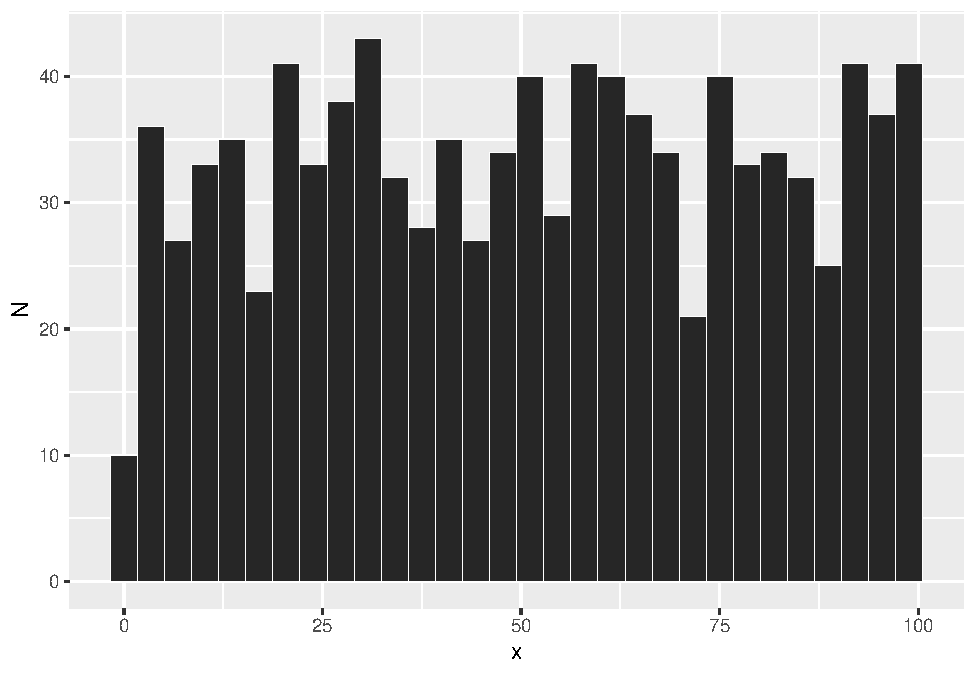
\includegraphics{_main_files/figure-latex/unnamed-chunk-34-1} 

}

\caption{Uniform Population Distribution (N = 1000)}\label{fig:unnamed-chunk-34}
\end{figure}

As expected, these randomly generated data are uniformly distributed. Next, we will draw 100 random samples of various sizes and plot the average of each.

\begin{Shaded}
\begin{Highlighting}[]
\CommentTok{# Define number of samples to draw from population distribution}
\NormalTok{samples <-}\StringTok{ }\DecValTok{100}

\CommentTok{# Populate vector with sample sizes}
\NormalTok{sample_n <-}\StringTok{ }\KeywordTok{c}\NormalTok{(}\DecValTok{1}\OperatorTok{:}\DecValTok{5}\NormalTok{,}\DecValTok{10}\NormalTok{,}\DecValTok{25}\NormalTok{,}\DecValTok{50}\NormalTok{)}

\CommentTok{# Initialize empty data frame to hold sample means}
\NormalTok{sample_means =}\StringTok{ }\OtherTok{NULL}

\CommentTok{# Set seed for reproducible random samples}
\KeywordTok{set.seed}\NormalTok{(}\DecValTok{456}\NormalTok{)}

\CommentTok{# For each n, draw random samples}
\ControlFlowTok{for}\NormalTok{ (n }\ControlFlowTok{in}\NormalTok{ sample_n) \{}
  
  \ControlFlowTok{for}\NormalTok{ (draw }\ControlFlowTok{in} \DecValTok{1}\OperatorTok{:}\NormalTok{samples) \{}
    
      \CommentTok{# Store sample means in data frame}
\NormalTok{      sample_means <-}\StringTok{ }\KeywordTok{rbind}\NormalTok{(sample_means, }\KeywordTok{cbind.data.frame}\NormalTok{(}
                            \DataTypeTok{n =}\NormalTok{ n, }
                            \DataTypeTok{x_bar =} \KeywordTok{mean}\NormalTok{(}\KeywordTok{sample}\NormalTok{(rand.unif, n, }\DataTypeTok{replace =} \OtherTok{TRUE}\NormalTok{, }\DataTypeTok{prob =} \OtherTok{NULL}\NormalTok{))))}
\NormalTok{  \}}
\NormalTok{\}}

\CommentTok{# Produce histograms to visualize distributions of sample means, grouped by n-count}
\NormalTok{sample_means }\OperatorTok\StringTok{ }\KeywordTok{ggplot}\NormalTok{() }\OperatorTok{+}\StringTok{ }
\StringTok{  }\KeywordTok{aes}\NormalTok{(}\DataTypeTok{x =}\NormalTok{ x_bar, }\DataTypeTok{fill =}\NormalTok{ n) }\OperatorTok{+}\StringTok{ }
\StringTok{  }\KeywordTok{labs}\NormalTok{(}\DataTypeTok{x =} \StringTok{"x-bar"}\NormalTok{, }\DataTypeTok{y =} \StringTok{"n"}\NormalTok{) }\OperatorTok{+}\StringTok{ }
\StringTok{  }\KeywordTok{geom_histogram}\NormalTok{(}\DataTypeTok{colour =} \StringTok{"white"}\NormalTok{, }\DataTypeTok{size =} \FloatTok{.1}\NormalTok{, }\DataTypeTok{fill =} \StringTok{"#262626"}\NormalTok{) }\OperatorTok{+}\StringTok{ }
\StringTok{  }\KeywordTok{facet_wrap}\NormalTok{(}\OperatorTok{~}\NormalTok{n)}
\end{Highlighting}
\end{Shaded}

\begin{figure}

{\centering 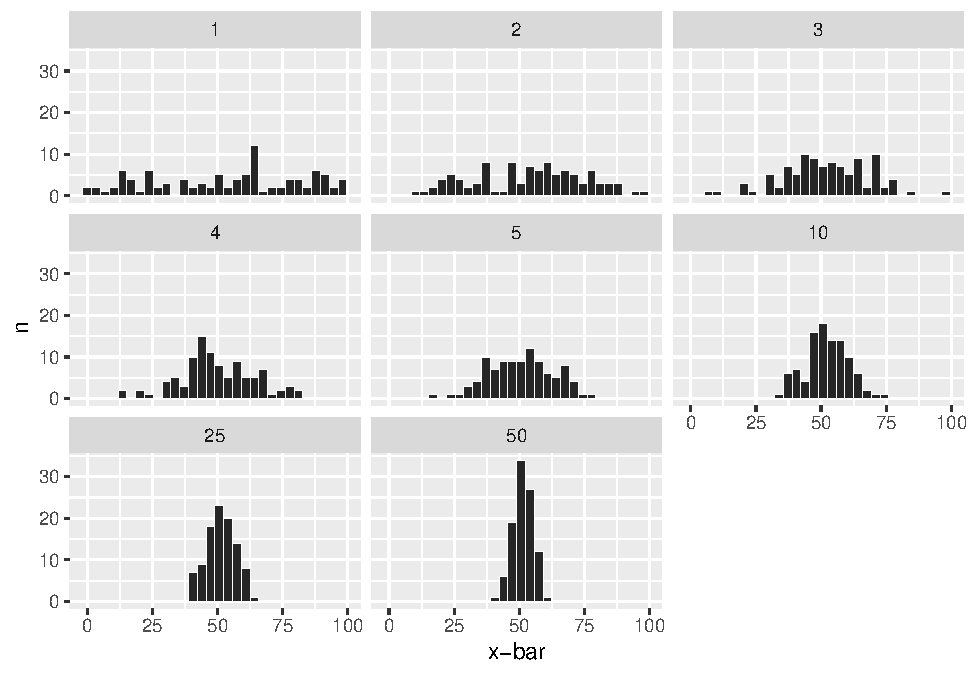
\includegraphics{_main_files/figure-latex/unnamed-chunk-35-1} 

}

\caption{Distribution of 100 Sample Means of Varied Size}\label{fig:unnamed-chunk-35}
\end{figure}

Per the CLT, we can see that as n increases, the sample means become more normally distributed.

\hypertarget{confidence-intervals}{%
\subsection{Confidence Intervals}\label{confidence-intervals}}

A \textbf{Confidence Interval (CI)} represents a range of values likely to include a population parameter of interest (usually \(\mu\)). A related concept that is fundamental to estimating CIs is the \textbf{standard error (SE)}, which is the standard deviation of sample means. While the standard deviation is a measure of variability for random variables, the variability captured by the SE reflects how representative the sample is of the population. Since sample statistics will approach the actual population parameters as the size of the sample increases, the SE and sample size are inversely related; that is, the SE decreases as the sample size increases. The SE is defined by:

\[ SE = \frac{\sigma}{\sqrt{n}} \]

Next, let's validate that our simulated distribution of sample means adheres to the properties of normally distributed data per the Empirical Rule:

\begin{Shaded}
\begin{Highlighting}[]
\CommentTok{# Store sample means with n = 50}
\NormalTok{x_bars <-}\StringTok{ }\NormalTok{sample_means[sample_means}\OperatorTok{$}\NormalTok{n }\OperatorTok{==}\StringTok{ }\DecValTok{50}\NormalTok{, }\StringTok{"x_bar"}\NormalTok{]}

\CommentTok{# Store sample size}
\NormalTok{n <-}\StringTok{ }\KeywordTok{length}\NormalTok{(x_bars)}

\CommentTok{# Calculate percent of sample means within +/- 2 SEs}
\KeywordTok{length}\NormalTok{(x_bars[x_bars }\OperatorTok{<}\StringTok{ }\KeywordTok{mean}\NormalTok{(x_bars) }\OperatorTok{+}\StringTok{ }\DecValTok{2} \OperatorTok{*}\StringTok{ }\KeywordTok{sd}\NormalTok{(x_bars) }\OperatorTok{&}\StringTok{ }\NormalTok{x_bars }\OperatorTok{>}\StringTok{ }\KeywordTok{mean}\NormalTok{(x_bars) }\OperatorTok{-}\StringTok{ }\DecValTok{2} \OperatorTok{*}\StringTok{ }\KeywordTok{sd}\NormalTok{(x_bars)]) }\OperatorTok{/}\StringTok{ }\NormalTok{n }\OperatorTok{*}\StringTok{ }\DecValTok{100}
\end{Highlighting}
\end{Shaded}

\begin{verbatim}
## [1] 97
\end{verbatim}

97\% of sample means are within 2 SEs, which is roughly what we expect per the characteristics of the normal distribution.

\begin{Shaded}
\begin{Highlighting}[]
\CommentTok{# Calculate percent of sample means within +/- 3 SEs}
\KeywordTok{length}\NormalTok{(x_bars[x_bars }\OperatorTok{<}\StringTok{ }\KeywordTok{mean}\NormalTok{(x_bars) }\OperatorTok{+}\StringTok{ }\DecValTok{3} \OperatorTok{*}\StringTok{ }\KeywordTok{sd}\NormalTok{(x_bars) }\OperatorTok{&}\StringTok{ }\NormalTok{x_bars }\OperatorTok{>}\StringTok{ }\KeywordTok{mean}\NormalTok{(x_bars) }\OperatorTok{-}\StringTok{ }\DecValTok{3} \OperatorTok{*}\StringTok{ }\KeywordTok{sd}\NormalTok{(x_bars)]) }\OperatorTok{/}\StringTok{ }\NormalTok{n }\OperatorTok{*}\StringTok{ }\DecValTok{100}
\end{Highlighting}
\end{Shaded}

\begin{verbatim}
## [1] 100
\end{verbatim}

All of the sample means are within 3 SEs, indicating that it would be highly unlikely -- nearly impossible even -- to observe a sample mean `from the same population' that falls outside this interval.

Now, let's illustrate the relationship between CIs and standard errors using sample data from our uniform population distribution. In our example, both \(\mu\) and \(\sigma\) are known and our sample size \(n\) is at least 30; therefore, we can use a \textbf{Z-Test} to calculate the 95\% CI. A \(z\) score of 1.96 corresponds to the 95\% CI -- the range of values we would expect to include \(\mu\) in at least 95 of 100 random samples taken from the population:

The CI in this case is defined by:

\[ CI = \bar{X} \pm z \frac{\sigma}{\sqrt{n}} \]

Let's randomly take \(n\) = 100 from the population, and compute sample statistics to estimate the 95\% CI:

\begin{Shaded}
\begin{Highlighting}[]
\CommentTok{# Set seed for reproducible random samples}
\KeywordTok{set.seed}\NormalTok{(}\DecValTok{456}\NormalTok{)}

\CommentTok{# Sample 100 values from uniform population distribution}
\NormalTok{x <-}\StringTok{ }\KeywordTok{sample}\NormalTok{(rand.unif, }\DecValTok{100}\NormalTok{, }\DataTypeTok{replace =} \OtherTok{TRUE}\NormalTok{, }\DataTypeTok{prob =} \OtherTok{NULL}\NormalTok{)}

\CommentTok{# Calculate 95% CI}
\NormalTok{ci95_lower_bound <-}\StringTok{ }\KeywordTok{mean}\NormalTok{(x) }\OperatorTok{-}\StringTok{ }\FloatTok{1.96} \OperatorTok{*}\StringTok{ }\NormalTok{(}\KeywordTok{sd}\NormalTok{(x) }\OperatorTok{/}\StringTok{ }\KeywordTok{sqrt}\NormalTok{(}\DecValTok{100}\NormalTok{))}
\NormalTok{ci95_upper_bound <-}\StringTok{ }\KeywordTok{mean}\NormalTok{(x) }\OperatorTok{+}\StringTok{ }\FloatTok{1.96} \OperatorTok{*}\StringTok{ }\NormalTok{(}\KeywordTok{sd}\NormalTok{(x) }\OperatorTok{/}\StringTok{ }\KeywordTok{sqrt}\NormalTok{(}\DecValTok{100}\NormalTok{))}
\end{Highlighting}
\end{Shaded}

\begin{Shaded}
\begin{Highlighting}[]
\CommentTok{# Print lower bound for 95% CI}
\NormalTok{ci95_lower_bound}
\end{Highlighting}
\end{Shaded}

\begin{verbatim}
## [1] 47.90733
\end{verbatim}

\begin{Shaded}
\begin{Highlighting}[]
\CommentTok{# Print upper bound for 95% CI}
\NormalTok{ci95_upper_bound}
\end{Highlighting}
\end{Shaded}

\begin{verbatim}
## [1] 58.98773
\end{verbatim}

Our known \(\mu\) is 51.2, which is covered by our 95\% CI (47.9 - 59.0). Per the CLT, in less than 5\% of cases would we expect to draw a random sample from the population that results in a 95\% CI which does not include \(\mu\). Note that our CI narrows with larger samples since our confidence that the range includes \(\mu\) increases with more data.

Next, let's look at a 99\% CI. We will enter 2.576 for \(z\):

\begin{Shaded}
\begin{Highlighting}[]
\CommentTok{# Calculate 99% CI}
\NormalTok{ci99_lower_bound <-}\StringTok{ }\KeywordTok{mean}\NormalTok{(x) }\OperatorTok{-}\StringTok{ }\FloatTok{2.576} \OperatorTok{*}\StringTok{ }\NormalTok{(}\KeywordTok{sd}\NormalTok{(x) }\OperatorTok{/}\StringTok{ }\KeywordTok{sqrt}\NormalTok{(}\DecValTok{100}\NormalTok{))}
\NormalTok{ci99_upper_bound <-}\StringTok{ }\KeywordTok{mean}\NormalTok{(x) }\OperatorTok{+}\StringTok{ }\FloatTok{2.576} \OperatorTok{*}\StringTok{ }\NormalTok{(}\KeywordTok{sd}\NormalTok{(x) }\OperatorTok{/}\StringTok{ }\KeywordTok{sqrt}\NormalTok{(}\DecValTok{100}\NormalTok{))}
\end{Highlighting}
\end{Shaded}

\begin{Shaded}
\begin{Highlighting}[]
\CommentTok{# Print lower bound for 99% CI}
\NormalTok{ci99_lower_bound}
\end{Highlighting}
\end{Shaded}

\begin{verbatim}
## [1] 46.16612
\end{verbatim}

\begin{Shaded}
\begin{Highlighting}[]
\CommentTok{# Print upper bound for 99% CI}
\NormalTok{ci99_upper_bound}
\end{Highlighting}
\end{Shaded}

\begin{verbatim}
## [1] 60.72893
\end{verbatim}

Like the 95\% CI, this slightly wider 99\% CI (46.2 - 60.7) also includes our \(\mu\) of 51.2.

If \(\sigma\) is not known, and/or we have a small sample (\(n\) \textless{} 30), we need to use a \textbf{T-Test} to calculate the CIs. In a people analytics setting, the reality is that population parameters are often unknown. For example, if we knew how engagement scores vary in the employee population, there would be no need to survey a sample of employees and make inferences about said population.

As we will see, the T-Test underpins many statistical tests and models germane to the people analytics discipline since we are often working with small datasets, so it is important to understand the mechanics. The \(t\) distribution is wider and shorter relative to the normal distribution, and this is characteristic of the distribution of sample means for smaller samples we observed in our CLT example. As a result, we must apply a different factor to estimate the CI to reflect the more \textbf{platykurtic} distribution. The CI in this case is defined by:

\[ CI = \bar{X} \pm t \frac{\sigma}{\sqrt{n}} \]

Let's compare CIs calculated using a T-Test to those calculated using the Z-Test. While a fixed \(z\) score can be used for each CI level when \(n\) \textgreater{} 30, the \(t\) statistic varies based on both the CI level and \textbf{degrees of freedom (df)} (\(n\) - 1). We can reference the following table to obtain the \(t\) statistic for each CI level:

\begin{figure}

{\centering 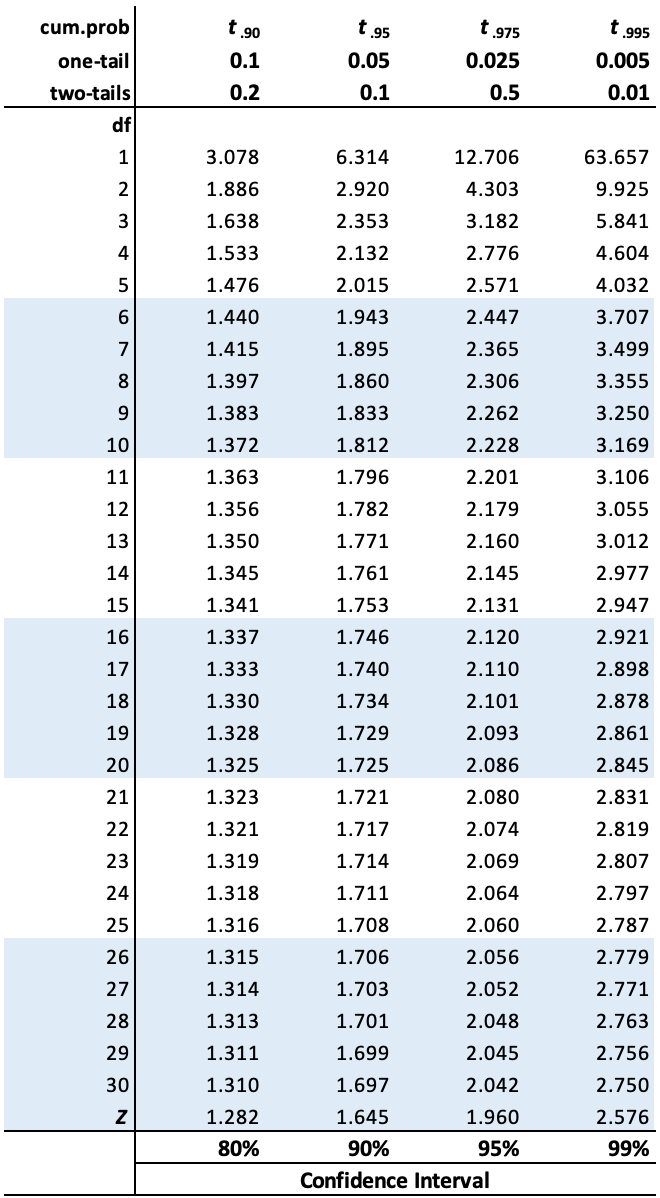
\includegraphics[width=9.17in]{/Users/craig.starbuck/Library/Mobile Documents/com~apple~CloudDocs/Documents/People Analytics Book/GitHub/peopleanalytics_lifecycle_book/graphics/t-table} 

}

\caption{Critical Values of Student's t Distribution}\label{fig:unnamed-chunk-44}
\end{figure}

For illustrative purposes, let's draw a smaller sample of \(n\) = 25 from our uniform population distribution and calculate the 95\% CI using the \(t\) statistic from the table (\(df\) = 24):

\begin{Shaded}
\begin{Highlighting}[]
\CommentTok{# Set seed for reproducible random samples}
\KeywordTok{set.seed}\NormalTok{(}\DecValTok{456}\NormalTok{)}

\CommentTok{# Sample 25 values from uniform population distribution}
\NormalTok{x <-}\StringTok{ }\KeywordTok{sample}\NormalTok{(rand.unif, }\DecValTok{25}\NormalTok{, }\DataTypeTok{replace =} \OtherTok{TRUE}\NormalTok{, }\DataTypeTok{prob =} \OtherTok{NULL}\NormalTok{)}

\CommentTok{# Calculate 95% CI}
\NormalTok{ci95_lower_bound <-}\StringTok{ }\KeywordTok{mean}\NormalTok{(x) }\OperatorTok{-}\StringTok{ }\FloatTok{2.064} \OperatorTok{*}\StringTok{ }\NormalTok{(}\KeywordTok{sd}\NormalTok{(x) }\OperatorTok{/}\StringTok{ }\KeywordTok{sqrt}\NormalTok{(}\DecValTok{25}\NormalTok{))}
\NormalTok{ci95_upper_bound <-}\StringTok{ }\KeywordTok{mean}\NormalTok{(x) }\OperatorTok{+}\StringTok{ }\FloatTok{2.064} \OperatorTok{*}\StringTok{ }\NormalTok{(}\KeywordTok{sd}\NormalTok{(x) }\OperatorTok{/}\StringTok{ }\KeywordTok{sqrt}\NormalTok{(}\DecValTok{25}\NormalTok{))}
\end{Highlighting}
\end{Shaded}

\begin{Shaded}
\begin{Highlighting}[]
\CommentTok{# Print lower bound for 95% CI}
\NormalTok{ci95_lower_bound}
\end{Highlighting}
\end{Shaded}

\begin{verbatim}
## [1] 35.24305
\end{verbatim}

\begin{Shaded}
\begin{Highlighting}[]
\CommentTok{# Print upper bound for 95% CI}
\NormalTok{ci95_upper_bound}
\end{Highlighting}
\end{Shaded}

\begin{verbatim}
## [1] 59.60959
\end{verbatim}

As expected, the 95\% CI using the \(t\) statistic is much wider (35.2 - 59.6), acknowledging the increased uncertainty in estimating population parameters given this smaller sample. To increase our confidence to the 99\% level, the interval widens even further (30.9 - 63.9):

\begin{Shaded}
\begin{Highlighting}[]
\CommentTok{# Calculate 99% CI}
\NormalTok{ci99_lower_bound <-}\StringTok{ }\KeywordTok{mean}\NormalTok{(x) }\OperatorTok{-}\StringTok{ }\FloatTok{2.797} \OperatorTok{*}\StringTok{ }\NormalTok{(}\KeywordTok{sd}\NormalTok{(x) }\OperatorTok{/}\StringTok{ }\KeywordTok{sqrt}\NormalTok{(}\DecValTok{25}\NormalTok{))}
\NormalTok{ci99_upper_bound <-}\StringTok{ }\KeywordTok{mean}\NormalTok{(x) }\OperatorTok{+}\StringTok{ }\FloatTok{2.797} \OperatorTok{*}\StringTok{ }\NormalTok{(}\KeywordTok{sd}\NormalTok{(x) }\OperatorTok{/}\StringTok{ }\KeywordTok{sqrt}\NormalTok{(}\DecValTok{25}\NormalTok{))}
\end{Highlighting}
\end{Shaded}

\begin{Shaded}
\begin{Highlighting}[]
\CommentTok{# Print lower bound for 99% CI}
\NormalTok{ci99_lower_bound}
\end{Highlighting}
\end{Shaded}

\begin{verbatim}
## [1] 30.91633
\end{verbatim}

\begin{Shaded}
\begin{Highlighting}[]
\CommentTok{# Print upper bound for 99% CI}
\NormalTok{ci99_upper_bound}
\end{Highlighting}
\end{Shaded}

\begin{verbatim}
## [1] 63.93631
\end{verbatim}

\textbf{Hypothesis Testing}

\textbf{Hypothesis testing} is how we leverage CIs to test whether a significant difference or relationship exists in the data. Sir Ronald Fisher invented what is known as the null hypothesis, which states that there is no relationship/difference; disprove me if you can! The null hypothesis is defined by:

\[ H_0: \mu_A = \mu_B \]

The objective of hypothesis testing is to determine if there is sufficient evidence to reject the null hypothesis in favor of an alternative hypothesis. The null hypothesis always states that there is `nothing' of significance. For example, if we want to test whether an intervention has an effect on an outcome in a population, the null hypothesis states that there is no effect. If we want to test whether there is a difference in average scores between two groups in a population, the null hypothesis states that there is no difference.

An alternative hypothesis may simply state that there is a difference or relationship in the population, or it may specify the expected direction (e.g., Population A has a significantly `larger' or `smaller' average value than Population B; Variable A is `positively' or `negatively' related to Variable B). Therefore, alternative hypotheses are defined by:

\[ H_A: \mu_A \neq \mu_B \]

\[ H_A: \mu_A < \mu_B \]

\[ H_A: \mu_A > \mu_B \]

\textbf{Alpha}

The \textbf{alpha} level of a hypothesis test, denoted by \(\alpha\), represents the probability of obtaining observed results due to chance if the null hypothesis is true. In other words, \(\alpha\) is the probability of rejecting the null hypothesis (and therefore claiming that there is a significant difference or relationship) when in fact we should have failed to reject it because there is insufficient evidence to support the alternative hypothesis.

\(\alpha\) is often set at .05 but is sometimes set at a more rigorous .01, depending upon the context and tolerance for error. An \(\alpha\) of .05 corresponds to a 95\% CI (1 - .05), and .01 to a 99\% CI (1 - .01). With non-directional alternative hypotheses, we must divide \(\alpha\) by 2 (i.e., we could observe a significant result in either tail of the distribution), while one-tailed tests position the rejection region entirely within one tail based on what is being hypothesized.

At the .05 level, we would conclude that a finding is statistically significant if the chance of observing a value at least as extreme as the one observed is less than 1 in 20 if the null hypothesis is true. Note that we observed this behavior with our simulated distribution of sample means. While we could observe more extreme values by chance with repeated attempts, in less than 1 in every 20 times would we expect a 95\% CI that does not capture \(\mu\). Moreover, in less than 1 in every 100 times should we expect a sample with a 99\% CI that does not capture \(\mu\).

\textbf{Beta}

Another key value is \textbf{Beta}, denoted by \(\beta\), which relates to the power of the analysis. Simply put, power reflects our ability to find a difference or relationship if there is one. Power is calculated by 1 - \(\beta\). At this point, it should be intuitive that larger samples increase our chances of observing significant results. As we observed in the T-Test example, CIs for small samples (\(n\) \textless{} 30) are quite wide relative to those for large samples; therefore, the power of the analysis to detect significance is limited given how extremely different values of \(x\) must be to observe non-overlapping CIs.

\textbf{Type I \& II Errors}

A \textbf{Type I Error} is a false positive, wherein we conclude that there is a significant difference or relationship when there is not. A \textbf{Type II Error} is a false negative, wherein we fail to capture a significant finding. \(\alpha\) represents our chance of making a Type I Error, while \(\beta\) represents our chance of making a Type II Error. I once had a professor explain that committing a Type I error is a shame, while committing a Type II error is a pity, and I've found this to be a helpful way to remember what each type of error represents.

\begin{figure}

{\centering 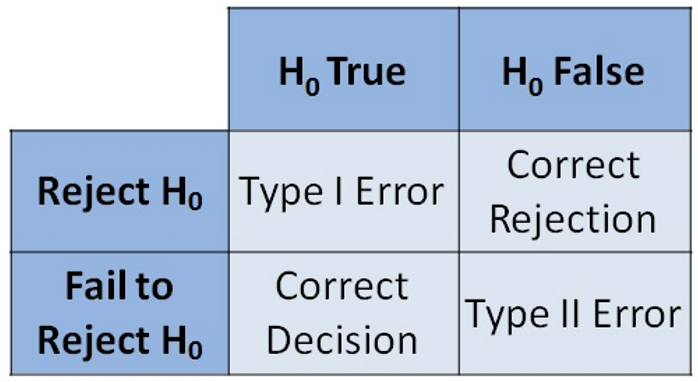
\includegraphics[width=12.42in]{/Users/craig.starbuck/Library/Mobile Documents/com~apple~CloudDocs/Documents/People Analytics Book/GitHub/peopleanalytics_lifecycle_book/graphics/hypothesis_testing_errors} 

}

\caption{Type I and II Errors}\label{fig:unnamed-chunk-51}
\end{figure}

\textbf{P-Values}

In statistical tests, the \textbf{p-value} is referenced to determine whether the null hypothesis can be rejected. The p-value represents the probability of obtaining a result at least as extreme as the one observed if the null hypothesis is true. As a general rule, if \(p\) \textless{} .05, we can confidently reject the null hypothesis and conclude that the observed difference or relationship was unlikely a chance observation.

While statistical significance helps us understand the probability of observing results by chance when there is actually no difference or effect in the population, it does not tell us anything about the size of the difference or effect. Analysis should never be reduced to inspecting p-values; in fact, p-values have been the subject of much controversy among researchers and practitioners in recent years. Later chapters will cover how to interpret results of statistical tests to surface the story and determine if there is anything `practically' significant among statistically significant findings.

\textbf{Bonferroni Correction}

One caveat when leveraging a p-value to determine statistical significance is that when multiple testing is performed -- that is, multiple tests using the same sample data -- the probability of a Type I error increases by a factor equivalent to the number of tests performed. It's important to note that there is not agreement among statisticians about how (or even whether) the p-value threshold for statistical significance needs to be adjusted to account for this increased risk. Nevertheless, we will cover this conservative approach for mitigating this risk.

Thus far, we have only discussed statistical significance in the context of a \textbf{per analysis error rate} -- that is, the probability of committing a Type I error for a single statistical test. However, when two or more tests are being conducted on the same sample, the \textbf{familywise error rate} is an important factor in determining statistical significance. The familywise error rate reflects the fact that as we conduct more and more analyses on the same sample, the probability of a Type I error across the set (or family) of analyses increases. The familywise error rate can be calculated by:

\[ \alpha_{FW} = 1 - (1 - \alpha_{PC})^C,  \]

where \(c\) is equal to the number of comparisons (or statistical tests) performed, and \(\alpha_{PC}\) is equal to the specified per analysis error rate (usually .05). For example, if \(\alpha\) = .05 per analysis, the probability of a Type I error with three tests on the same data increases from 5\% to 14.3\%: \(1 - (1 - .05)^3 = .143\).

The most common method of adjusting the familywise error rate down to the specified per analysis error rate is the \textbf{Bonferroni Correction}. To implement this correction, we can simply divide \(\alpha\) by the number of analyses performed on the dataset -- such as \(\alpha / 3 = .017\) in the case of three analyses with \(\alpha = .05\). This means that for each statistical test, we must achieve \(p < .017\) to report a statistically significant result. An alternative which allows us to achieve the same number of statistically significant results is to multiply the unadjusted per analysis p-values for each statistical test by the number of tests. For example, if we run three statistical tests and receive \(p = .014\), \(p = .047\), and \(p = .125\), we would achieve one significant result with the first method (\(p < .017\)) as well as with the alternative since the first statistical test satisfies the per analysis error rate (\(p < .05\)): \(p = .014 * 3 = .042\).

Perneger (1998) is one of many who oppose the use of the Bonferroni Correction, suggesting that these ``adjustments are, at best, unnecessary and, at worst, deleterious to sound statistical inference.'' The Bonferroni Correction is controversial among researchers because while applying the correction reduces the chance of a Type I error, it also increases the chance of a Type II error. Because this correction makes it more difficult to detect significant results, it is rare to find such a correction reported in published research, though research often involves multiple testing on the same sample. Perneger suggests that simply describing the statistical tests that were performed, and why, is sufficient for dealing with potential problems introduced by multiple testing.

\hypertarget{exercises}{%
\section{Exercises}\label{exercises}}

\begin{enumerate}
\def\labelenumi{\arabic{enumi}.}
\item
  Parameters are descriptions or characteristics of a sample, while statistics are descriptions or characteristics of a population.
  A. True
  B. False
\item
  Which of the following is an example of a null hypothesis, where ``µ'' reflects the mean of a population?
  A. µA = µB
  B. µA ≠ µB
  C. µA \textless{} µB
  D. µA \textgreater{} µB
  E. None of the above; all are examples of alternative hypotheses.
\item
  Which of the following describes a Type I Error?
  A. Failing to reject the null hypothesis when it is false
  B. Rejecting the null hypothesis when it is true
  C. Reporting something as significant when nothing of significance is present (a shame)
  D. Failing to detect something of significance (a pity)
  E. Both B and C
  F. Both A and D
\item
  100 randomly selected employees in the Marketing department of an organization participated in a survey on career pathing for marketing professionals. What is the sample and what is the population sampled in this case?
  A. Sample: 100 employees who completed the survey, Population: All employees in the organization
  B. Sample: 100 employees who completed the survey, Population: Marketing employees
  C. Sample: All Marketing professionals, Population: All employees in the organization
  D. Sample: All employees in the organization, Population: Employees across all companies globally
\item
  The primary purpose of inferential statistics is to make inferences about a population based on sample data. Inferential statistics allows these inferences to be made with defined levels of confidence that what is observed in a sample is also characteristic of the larger population.
  A. True
  B. False
\item
  The median tends to be a better measure of central tendency since the mean is more sensitive to extreme values (outliers)?
  A. True
  B. False
\item
  The standard deviation represents the `average' amount by which individual values for a variable deviate (or vary) from the mean. A large standard deviation indicates there is considerable spread in the data, whereas a small standard deviation indicates the mean is fairly representative of the data.
  A. True
  B. False
\item
  A positively skewed distribution has its largest allocation to the left and a negative distribution to the right.
  A. True
  B. False
\item
  The mean alone is sufficient for understanding the distribution of a set of data.
  A. True
  B. False
\item
  A T-Test should be used when \(\sigma\) is unknown and/or \(n\) \textless{} 30.
  A. True
  B. False
\end{enumerate}

\hypertarget{data-preparation}{%
\chapter{Data Preparation}\label{data-preparation}}

\hypertarget{data-wrangling}{%
\section{Data Wrangling}\label{data-wrangling}}

\hypertarget{feature-engineering}{%
\section{Feature Engineering}\label{feature-engineering}}

Level one people analytics tends to utilize only the delivered fields from the HRIS (e.g., location, job profile, org tenure, etc.), but a good next step is to derive smarter variables from these fields. These can then be used to slice and dice turnover and engagement data differently, use as inputs in attrition risk models, etc. Below are some ideas to get you started:

\begin{itemize}
\tightlist
\item
  Number of jobs per unit of tenure (larger proportions tend to see greater career pathing)
\item
  Office/remote worker (binary variable dummy coded as 1/0)
\item
  Local/remote manager (binary variable dummy coded as 1/0)
\item
  Hire/Rehire (binary variable dummy coded as 1/0)
\item
  Hired/acquired (proxy for culture shock effects)
\item
  Gender isolation (ratio of employee's gender to number of the same within immediate work
  group)
\item
  Generation isolation (comparison of age bracket to most frequent generational bracket within
  immediate work group)
\item
  Ethnic isolation (ratio of employee's ethnicity to number of the same within immediate work
  group)
\item
  Difference between employee and manager age
\item
  Percentage change between last two performance appraisal scores (per competency and/or
  overall)
\item
  Team and department quit outbreak indicators (ratio of terms over x months relative to average
  headcount over x months)
\item
  Industry experience (binary or length in years)
\end{itemize}

Remember to compute variables consistent with a need (e.g., is there reason to believe generationally isolated employees are more likely to term?). There may be a time and place for undertaking data mining initiatives with no a priori theories about what may be uncovered; however, more often than not, our efforts should be tied to specific hypotheses the business needs tested, which have sound theoretical underpinnings.

\hypertarget{analysis-of-differences}{%
\chapter{Analysis of Differences}\label{analysis-of-differences}}

\hypertarget{comparing-2-distributions}{%
\section{Comparing 2 Distributions}\label{comparing-2-distributions}}

\hypertarget{comparing-3-distributions}{%
\section{Comparing 3+ Distributions}\label{comparing-3-distributions}}

\hypertarget{inferential-models}{%
\chapter{Inferential Models}\label{inferential-models}}

It's important to draw a distinction between inferential and predictive models. Inferential models are highly interpretable and their utility is largely in understanding the nature and magnitude of the effect variables have on outcomes. Inferential models also lend to quantifying the extent to which we can generalize the observed effects to the larger population from which the sample was drawn. The objective in predictive modeling is to also to learn from patterns in historical data but for the purpose of achieving the most accurate predictions of future events -- even at the expense of interpretability. To be clear, this isn't to say that predictive models cannot be interpreted -- they certainly can -- but I've seen relatively few applications for predictive modeling in people analytics because models generally need to be highly interpretable to support action planning.

This chapter is dedicated to inferential models to support a working understanding of how to interpret model output and communicate clear, data-driven narratives that respect the nuance and noise characteristic of people data. The following chapter will provide an overview of predictive modeling frameworks.

\hypertarget{regression}{%
\section{Regression}\label{regression}}

Regression is perhaps the most important statistical learning technique for people analytics. If you have taken a statistics course at the undergraduate or graduate levels, you have surely already encountered it. Before diving into the math to understand the mechanics of regression, let's develop an intuitive understanding.

Imagine we are sitting at a large public park in NYC on a nice fall afternoon. If asked to estimate the annual compensation of the next person to walk by, in the absence of any additional information how would you estimate this? Most would likely estimate the average annual compensation of everyone capable of walking by. Since this would include both residents and visitors, this would be a very large group of people! The obvious limitation with this approach is that among the large group of people capable of walking by, there is likely a significant range of annual compensation values. Many walking by may be children, unemployed, or retirees who earn no annual compensation, while others may be highly compensated senior executives at the pinnacle of their careers. Since the range of annual compensation could be zero to billions of dollars, estimating the average of such a large population is likely going to be highly inaccurate without more information about who may walk by.

Let's consider that we are sitting outside on a weekday afternoon. Should this influence our annual compensation estimate? It is likely that we can eliminate a large segment of those likely to walk by, as we would expect most children to be in school on a typical fall weekday afternoon. It's also unlikely that those who are employed and not on vacation will walk by on a fall weekday afternoon. Therefore, factoring in that it is a weekday should limit the size of the population which in turn may reduce the range of annual compensation values for our population of passerbys.

Let's now consider that the park is open only to invited guests for a symposium on people analytics. Though it may be difficult to believe, a relatively small subset of the population is likely interested in attending such a symposium, so this information will likely be very helpful in reducing the size of the population who could walk by, which should further reduce the range of annual compensation since we probably have a good idea of the profile of those most likely to attend. This probably also lessens (or altogether eliminates) the importance of the weekday factor in explaining why people vary in the amount of compensation they earn each year.

Furthermore, let's consider that only those who reside in NYC and Boise were invited, and that the next person to walk by resides in Boise. Most companies apply a significant cost of living multiplier to the compensation for those in an expensive region such as NYC, resulting in a significant difference in compensation relative to those residing in a much less expensive city like Boise -- all else being equal. Therefore, if we can partition attendees into two groups based on their geography, this should limit the range of annual compensation significantly within each -- likely making the average compensation amount in each group a more nuanced and reasonable estimate.

What if we also learn the specific zip code in which the next passerby from Boise resides? The important information is likely captured in the larger city label (NYC vs.~Boise), and the compensation for the specific zip codes within each city are unlikely to vary to a significant degree. Assuming this is true, it probably would not make sense to consider both the city name and zip code since they are effectively redundant pieces of information with regard to explaining differences in annual compensation.

What if we learn that the next person to walk by will be wearing a blue shirt? Does this influence your estimate? Unless there is research to suggest shirt color and earnings are related, this information will likely not contribute any significant information to our understanding of why people vary in the amount of compensation they earn annually and should, therefore, not be considered.

You can probably think of many relevant variables that would help further narrow the range of annual compensation. These may include job, level, years of experience, education, location, among other factors. The main thing to understand is that for each group of observations with the same characteristics -- such as senior analysts with a graduate degree who reside in NYC -- there is a distribution of annual compensation. This distribution reflects unexplained variance. That is, we do not have information to explain why the compensation for each and every person is not the same and in social science contexts, it simply is not practical to explain 100 percent of the variance in outcomes. Two people may be similar on hundreds of factors (experience, education, skills) but one was simply a more effective negotiator when offered the same role and commanded a higher salary. It's likely we do not have data on salary negotiation ability so this information would leave us with unexplained variance in compensation. The goal is simply to identify the variables that provide the most information in helping us tighten the distribution so that estimating the average value will generally be an accurate estimate for those in the larger population with the same characteristics.

While we can generally improve our estimates with more relevant information (not shirt color or residential zip code in this case), it is important to understand that samples which are too small (n \textless{} 30) lend to anomalies; modeling noise in sparse data can result in models that are unlikely to generalize beyond the sample data. For example, if the only people from Boise to attend the people analytics symposium happen to be two ultra wealthy tech entrepreneurs who earn millions each year, it would not be appropriate to use this as the basis for our estimates of all future attendees from Boise. This is a phenomenon known as overfitting that will be covered later in this chapter.

This is the essence of regression modeling: find a limited number of variables which independently or jointly provide significant information that helps explain (by reducing) variance around the average value. As illustrated in this example, adding additional variables (information) can impact the importance of other variables or may offer no incremental information at all. In the subsequent sections, we will cover how to identify which variables are important and how to quantify the effect they have on the outcome.

\hypertarget{simple-linear-regression}{%
\section{Simple Linear Regression}\label{simple-linear-regression}}

\hypertarget{parameter-estimation}{%
\subsection{Parameter Estimation}\label{parameter-estimation}}

Ordinary Least Squares (OLS) is the most common method for estimating unknown parameters in a linear regression model.

\hypertarget{multiple-linear-regression}{%
\section{Multiple Linear Regression}\label{multiple-linear-regression}}

\hypertarget{moderation}{%
\subsection{Moderation}\label{moderation}}

\hypertarget{mediation}{%
\subsection{Mediation}\label{mediation}}

\hypertarget{polynomial-regression}{%
\section{Polynomial Regression}\label{polynomial-regression}}

\hypertarget{logistic-regression}{%
\section{Logistic Regression}\label{logistic-regression}}

Logistic regression is an excellent tool when the outcome is categorical. Logistic regression allows us to model the probability of different classes -- a type of modeling often referred to as classification. The context for classification can be binomial for two classes (e.g., active/inactive, promoted/not promoted), multinomial for multiple unordered classes (e.g., skills, job families), or ordinal for multiple ordered classes (e.g., survey items measured on a Likert scale, performance level).

\hypertarget{binomial}{%
\subsection{Binomial}\label{binomial}}

\hypertarget{multinomial}{%
\subsection{Multinomial}\label{multinomial}}

\hypertarget{ordinal}{%
\subsection{Ordinal}\label{ordinal}}

Proportional Odds Logistic Regression

\hypertarget{hierarchical-models}{%
\section{Hierarchical Models}\label{hierarchical-models}}

\hypertarget{predictive-models}{%
\chapter{Predictive Models}\label{predictive-models}}

\hypertarget{bias-variance-trade-off}{%
\section{Bias-Variance Trade-Off}\label{bias-variance-trade-off}}

\hypertarget{cross-validation}{%
\section{Cross-Validation}\label{cross-validation}}

\hypertarget{balancing-classes}{%
\section{Balancing Classes}\label{balancing-classes}}

\hypertarget{model-performance}{%
\section{Model Performance}\label{model-performance}}

\hypertarget{automated-machine-learning-automl}{%
\chapter{Automated Machine Learning (AutoML)}\label{automated-machine-learning-automl}}

\hypertarget{unsupervised-learning-models}{%
\chapter{Unsupervised Learning Models}\label{unsupervised-learning-models}}

\hypertarget{factor-analysis}{%
\section{Factor Analysis}\label{factor-analysis}}

\hypertarget{clustering}{%
\section{Clustering}\label{clustering}}

\hypertarget{data-visualization}{%
\chapter{Data Visualization}\label{data-visualization}}

\hypertarget{data-storytelling}{%
\chapter{Data Storytelling}\label{data-storytelling}}

\hypertarget{bibliography}{%
\chapter{Bibliography}\label{bibliography}}

Baron, R. M., \& Kenny, D. A. (1986). The moderator--mediator variable distinction in social psychological research: Conceptual, strategic, and statistical considerations. Journal of Personality and Social Psychology, 51(6), 1173--1182.

Creswell, J. W., \& Creswell, J. D. (2018). Research Design: Qualitative, Quantitative, and Mixed Methods Approaches (5th ed.). Los Angeles: Sage.

Daw, R. H., \& Pearson, E. S. (1972). Studies in the History of Probability and Statistics. XXX. Abraham De Moivre's 1733 Derivation of the Normal Curve: A Bibliographical Note. Biometrika, 59(3), 677--680. \url{https://doi.org/10.2307/2334818}

James, G., Witten, D., Hastie, T., \& Tibshirani, R. (2013). An Introduction to Statistical Learning: With Applications in R. New York: Springer.

Kahneman, D. (2011). Thinking, fast and slow. New York: Farrar, Straus and Giroux.

Kerlinger, F., \& Lee, H. (2000). Foundations of behavioral research (4th ed.). Melbourne: Wadsworth.

Perneger, T. V. (1998). What's wrong with Bonferroni adjustments. BMJ, 316(7139), 1236-1238.

Pishro-Nik, H. (2014). Introduction to Probability: Statistics and Random Processes. Blue Bell, PA: Kappa Research, LLC.

Wheelan, C. (2013). Naked Statistics: Stripping the Dread from the Data. New York: W.W. Norton.

\hypertarget{appendix}{%
\chapter{Appendix}\label{appendix}}

\hypertarget{exercise-solutions}{%
\section{Exercise Solutions}\label{exercise-solutions}}

Statistical Fundamentals

\begin{enumerate}
\def\labelenumi{\arabic{enumi}.}
\item
  Parameters are descriptions or characteristics of a sample, while statistics are descriptions or characteristics of a population.
  B. False
\item
  Which of the following is an example of a null hypothesis, where ``µ'' reflects the mean of a population?
  A. µA = µB
\item
  Which of the following describes a Type I Error?
  E. Both B and C
\item
  100 randomly selected employees in the Marketing department of an organization participated in a survey on career pathing for marketing professionals. What is the sample and what is the population sampled in this case?
  B. Sample: 100 employees who completed the survey, Population: Marketing employees
\item
  The primary purpose of inferential statistics is to make inferences about a population based on sample data. Inferential statistics allows these inferences to be made with defined levels of confidence that what is observed in a sample is also characteristic of the larger population.
  A. True
\item
  The median tends to be a better measure of central tendency since the mean is more sensitive to extreme values (outliers)?
  A. True
\item
  The standard deviation represents the `average' amount by which individual values for a variable deviate (or vary) from the mean. A large standard deviation indicates there is considerable spread in the data, whereas a small standard deviation indicates the mean is fairly representative of the data.
  A. True
\item
  A positively skewed distribution has its largest allocation to the left and a negative distribution to the right.
  A. True
\item
  The mean alone is sufficient for understanding the distribution of a set of data.
  B. False
\item
  A T-Test should be used when \(\sigma\) is unknown and/or \(n\) \textless{} 30.
  A. True
\end{enumerate}

\hypertarget{d-framework-1}{%
\section{4D Framework}\label{d-framework-1}}

\begin{figure}
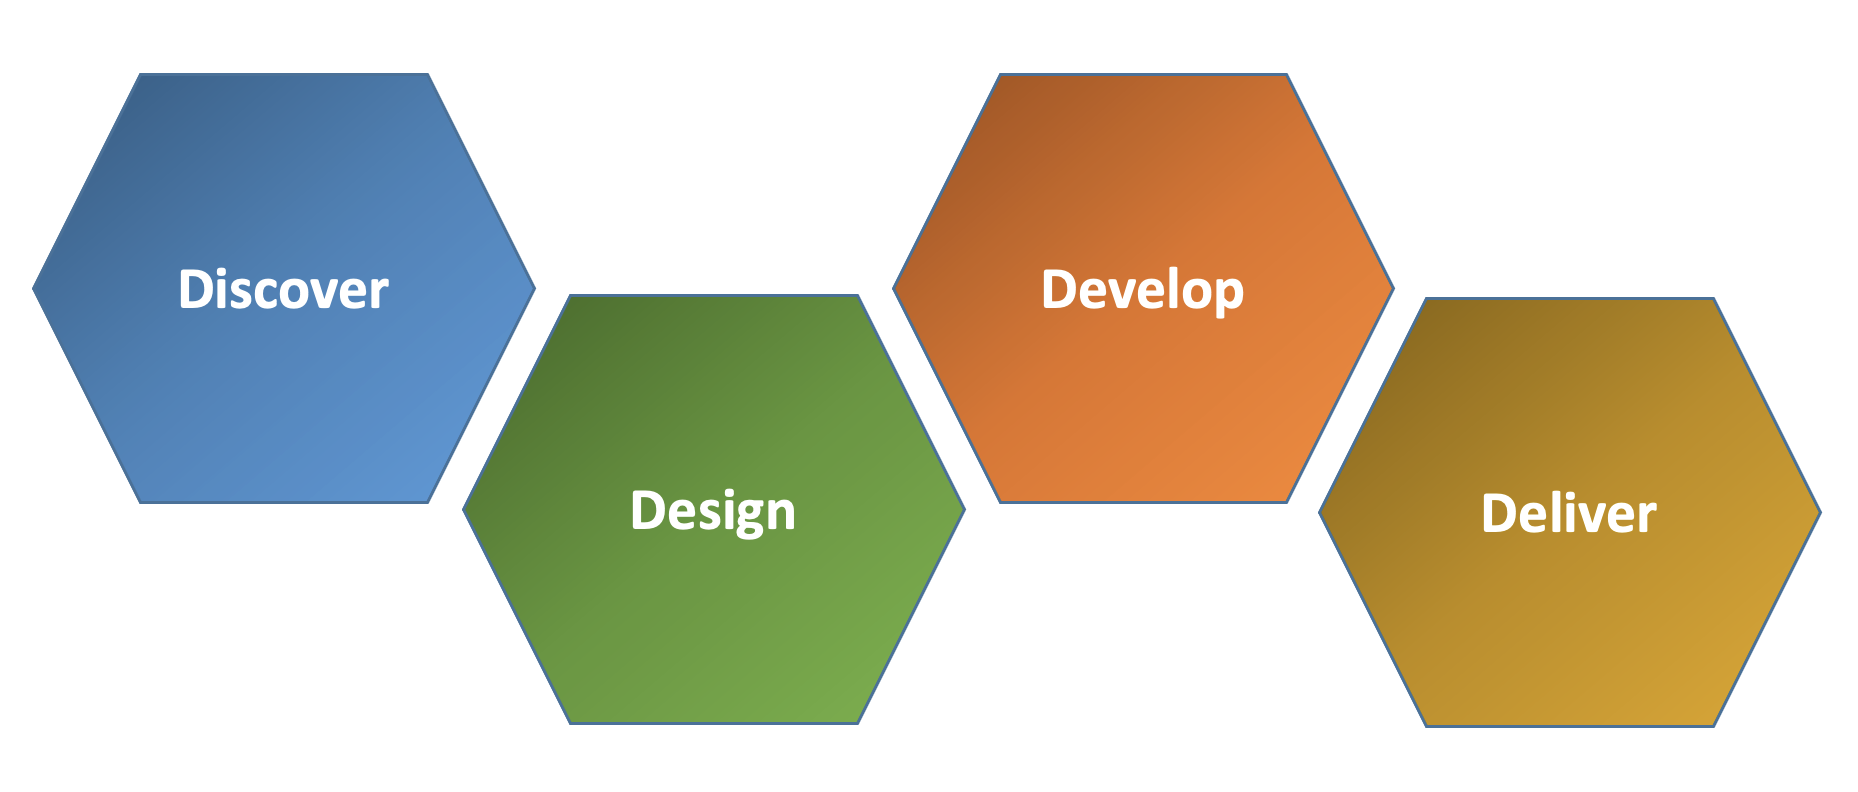
\includegraphics[width=25.81in]{/Users/craig.starbuck/Library/Mobile Documents/com~apple~CloudDocs/Documents/People Analytics Book/GitHub/peopleanalytics_lifecycle_book/graphics/4d_framework} \caption{Figure 1: 4D Framework}\label{fig:unnamed-chunk-52}
\end{figure}

1. Discover

You are likely familiar with the old adage: ``An ounce of prevention is worth a pound of cure.'' Such is the case with respect to planning in an analytics context. During the Discover phase, it is important to remain in the problem zone; seek to understand your clients' needs through active listening and questions. This is not the time for solutioning or committing to any specific deliverables. If the client's needs are ambiguous, proceeding will likely be an exercise in futility. Outlined below is a set of general questions that should be considered during this initial phase to prevent allocating scarce time and resourcing to a project that ultimately misses the mark.

\begin{itemize}
\item
  Client

  Who is the client? A client can be a person or organization that has contracting you for consulting services, or an internal stakeholder within your organization who has need. What is important to them?
\item
  Primary Objective

  \begin{itemize}
  \tightlist
  \item
    What is the client ultimately hoping to accomplish?
  \item
    Is the request merely to satisfy one's curiosity, or are there actions that can realistically be taken to materially influence said objective?
  \end{itemize}
\item
  Problem Statement

  \begin{itemize}
  \tightlist
  \item
    One of my most important early steps is clearly defining the problem statement. If your understanding of the problem -- after translating from the business terms in which it was initially expressed -- is misaligned with the client's needs, none of the subsequent steps matter.
  \end{itemize}
\item
  Guiding Theories

  \begin{itemize}
  \tightlist
  \item
    What theoretical explanations can the client offer as potential rationalizations for the phenomena of interest?
  \item
    Are there existing theories in the organizational literature that should guide how the problem is tackled (e.g., findings from similar research implemented in other contexts)?
  \end{itemize}
\item
  Research Questions

  To respect the nuances of the problem statement, it is important to unpack it and frame as a set of overarching questions to guide the research.

  \begin{itemize}
  \tightlist
  \item
    Q1: \ldots{}
  \item
    Q2: \ldots{}
  \item
    Q3: \ldots{}
  \end{itemize}
\item
  Research Hypotheses

  Once research questions are developed, what do you expect to find based on anecdotal stories or empirical findings? As a next step, these expectations should be expressed in the form of research hypotheses. Please note that these research hypotheses are different from statistical hypotheses.

  \begin{itemize}
  \tightlist
  \item
    H1: \ldots{}
  \item
    H2: \ldots{}
  \item
    H3: \ldots{}
  \end{itemize}

  To ensure the hypotheses lend themselves to actionable analyses, it is important to consider the following: ``What does success look like?'' In other words, once the project is complete, against which success measures will the project's success be determined? Curiosity is not a business reason and hope is not a reasonable strategy. The following questions may prove helpful in the promotion of actionable -- over merely interesting outcomes:

  \begin{itemize}
  \tightlist
  \item
    What will be done if the hypotheses are empirically supported?
  \item
    What will be done if the hypotheses are not empirically supported?
  \end{itemize}
\item
  Assumptions

  At this point, it's helpful to consider what assumptions may be embedded in this discovery work. Are the questions and hypotheses rooted in what the client has theorized, or are these the product of an ambiguous understanding of the client's needs?
\item
  Cadence

  \begin{itemize}
  \tightlist
  \item
    Is this analysis a one-off, or could there be a need to refresh this analysis on a regular cadence?
  \item
    Are there dates associated with programs, actions, etc. this analysis is intended to support?
  \end{itemize}
\item
  Aggregation

  Is there a need for individual-level detail supporting the analysis? Aaggregate data should generally be the default unless a compelling justification exists and approval from legal and privacy partners is granted. One important role of analysts is to help keep the audience focused on the bigger picture and findings. Access to individual-level detail can not only introduce unnecessary legal and compliance risk but can also lead to questions and probing that can delay taking needed actions based on the results.
\item
  Deliverable

  What is the preferred method of communicating the results of the analysis (e.g., interactive dashboard, static slide deck, document)? It is important to determine this early so that subsequent efforts can be structured to support the preferred deliverable. For example, if an interactive dashboard is preferred, does your Engineering department need to prioritize dependent tasks such as data feeds, row-level security, BI development, and production server migrations?
\item
  Filters \& Dimensions

  How does your client prefer to segment the workforce? Some common grouping dimensions are business unit, division, team, job family, location, tenure, and management level.
\end{itemize}

2. Design

Perhaps the most important initial question to answer in the design phase is: ``Does anything already exist that addresses part, or all, of the client's objectives?'' If the existing solution will suffice, it's possible that there is simply a communication/education gap, and you can allocate time and resources elsewhere.

The end-user experience is of paramount importance during the Design phase, as solutions should have a consistent look and feel regardless of who developed the product. To achieve this, it is important to resist siloed thinking and consider the broader set of analytics solutions the team has delivered -- or is in the process of delivering.

\begin{itemize}
\item
  Data Privacy

  Are there potential concerns with the study's objective, planned actions, and/or requested data elements from an employee privacy or legal perspective? A cross-functional data governance committee can help with efficient and consistent decisioning on requests for people data and analytics.
\item
  Data Sources \& Elements

  \begin{itemize}
  \tightlist
  \item
    What data sources are required?
  \item
    What data elements are required?
  \end{itemize}

  In cases where sensitive attributes such as gender, ethnicity, age, sexual orientation, and disability status are requested, it's always best to exercise a `safety first' mentality and consult with legal and privacy partners to ensure there is comfort with the intended use of the data. The decision on whether or not to include these sensitive data elements is often less about what the audience can view (e.g., People Partners may already have access to the information at the person level in the source system) and more anchored in what they plan to do with the information.

  Is the required data already accessible in a data warehouse or other analytics environment? If not, does it need to be? What is required to achieve this?
\item
  Data Quality

  It is important to understand the data generative process and never make assumptions about how anomalies or missing data should be interpreted. After identifying what data sources will be required for a particular analysis, it is important to meet with source system owners and data stewards to deeply understand the business processes by which data are generated in the system(s). Are there data quality concerns that need to be explored and addressed?
\item
  Variables

  How will the constructs be measured (e.g., survey instrument, derived attribute, calculated field)?
\item
  Analysis Method

  What are the appropriate analysis methods based on the research hypotheses? If modeling is required, is it more important to index on accuracy or interpretability?
\item
  Dependencies

  Are other teams required to develop this solution? What is the nature of the work each dependent team will perform? Are there required system configuration changes? Do these teams have capacity to support?
\item
  Change Management

  Will this solution impact current processes or solutions? If so, what is the change management plan to facilitate a seamless transition and user experience?
\item
  Sign-Off

  Generally, it is best for the client to signoff on the problem statement, analysis approach, and wire frame for the deliverable (if applicable) before providing an ETA and proceeding to the development phase. This ensures alignment on the client's needs and the perceived utility of the solution in addressing those needs.
\end{itemize}

3. Develop

\begin{itemize}
\item
  Development Patterns

  \begin{itemize}
  \tightlist
  \item
    Are there development patterns that should guide the development approach to support consistency?
  \item
    Are there existing calculated fields that can/should be leveraged for derived data?
  \item
    Are there best practices that should be employed to optimize performance (e.g., load time for dashboards, executing complex queries during non-peak times)?
  \item
    Are there standard color palettes that should be applied?
  \end{itemize}
\item
  Productionalizable Code

  \begin{itemize}
  \tightlist
  \item
    How do models and data science pipelines need to be developed to facilitate a seamless migration from lower to upper environments? For example, initial exploratory data analysis (EDA) may be performed using curated data in flat files for the purpose of identifying meaningful trends, relationships, and differences, but where will this data need to be sourced in production to automate the refresh of models at a regular interval? If the data were provided from multiple source systems, what joins are required to integrate the data? What transformation logic or business rules need to be applied to reproduce the curated data?
  \end{itemize}
\item
  Unit Testing

  \begin{itemize}
  \tightlist
  \item
    What test cases will ensure the veracity of data?
  \item
    Who will perform the testing?
  \end{itemize}
\item
  UAT Testing

  \begin{itemize}
  \tightlist
  \item
    In the spirit of agility and constant contact with the client to prevent surprises, it is generally a good idea to have the client take the solution for a test run within the UAT environment and then provide sign-off before migrating to production. If the deliverable is a deck or doc with results from a model, UAT may surface clarifying questions that can be addressed before releasing to the broader audience.
  \end{itemize}
\end{itemize}

4. Deliver

The Deliver phase can take many forms depending on the solution being released. If the solution is designed for a large user base, a series of recorded trainings may be in order so that there is a helpful reference for those unable to attend the live sessions or new joiners in the future. It is important to monitor success measures, which could be insights aligned to research hypotheses, dashboard utilization metrics, or any number of others defined within the Discover phase.

\bibliography{book.bib}

\end{document}
